% =============================================================
%  Active power decoupling of a single-phase AFE with a ripple port:
%  the method implemented in the model single_phase_afe of pwr-control/modelization-and-control
%  pwr-control documentation - compile with pdflatex (three times) from inside this folder:
%      pdflatex single_phase_afe_power_decoupling.tex
%  Figures: TikZ / circuitikz drawn in this file, plus the PDF figures of figures/ produced by
%  single_phase_afe_design_check.py (the same script as claude_analysis/ of the model folder).
%  The same source is kept in pwr-control/library (library/documentation/single_phase_afe_power_decoupling/),
%  where ../../AAA_template_latex_settings/ is a copy of the template of this repository.
% =============================================================
\documentclass[11pt,a4paper]{scrartcl}
\ifdefined\PWRCONTROLSETTINGSLOADED
\endinput
\fi
\def\PWRCONTROLSETTINGSLOADED{1}
% ===================== PACKAGES =====================
\usepackage[british]{babel}
\usepackage[tmargin=1in, bmargin=1in, lmargin=0.75in, rmargin=0.75in]{geometry}
\usepackage[dvipsnames,table]{xcolor}  % prima di tikz, listings, ecc.

\usepackage{tikz}
\usepackage{graphicx}
\usepackage{pgfplots}
\pgfplotsset{width=12cm, compat=1.9}
\usepackage{setspace}
\usepackage{chemmacros}
\usepackage{chemfig}
\usepackage{tabularray}
\usepackage{makeidx}
\usepackage{epstopdf}
\usepackage{amssymb}
\usepackage{mathrsfs}
\usepackage{bm}
\usepackage{amsmath}
% esint deve essere caricato DOPO amsmath: entrambi definiscono \iint, \iiint,
% \iiiint e \idotsint. Le si rende indefinite in modo che esint le ridefinisca
% (versioni con i simboli di integrale multiplo corretti) senza errori.
\let\iint\undefined
\let\iiint\undefined
\let\iiiint\undefined
\let\idotsint\undefined
\usepackage{esint}
\usepackage{enumitem}
%\usepackage[english]{varioref}
\usepackage{physics}
\usepackage{lipsum}
\usepackage{fancyhdr}
\usepackage{float}
\usepackage{empheq}
\usepackage[framemethod=tikz]{mdframed}
\numberwithin{equation}{section}
\usepackage{eso-pic}
\usepackage{calc}
\usepackage{nccmath}
\usepackage{caption}
\usepackage{subcaption}
\usepackage{gensymb}
\usepackage{amsfonts, amsthm, epsfig, epstopdf, titling, url, array}
\usepackage{tabularx}
\usepackage{makecell}
\usepackage{booktabs}
\usepackage{array}
\usepackage{siunitx}
\sisetup{input-digits=0123456789\pi}
\usepackage[symbol]{footmisc}
\usepackage{multicol}
%\usepackage{boondox-cal}
\usepackage{blindtext}
\usepackage{changepage}
\usepackage{nomencl}
\usepackage{hyperref}
\usepackage{xurl}
\usepackage{ragged2e}
\usepackage[version=4]{mhchem}  % ← conflitto di opzioni
\usepackage{longtable}
\usepackage{chemformula}
\usetikzlibrary{arrows.meta,positioning,calc}
\usepackage[page,toc]{appendix}


% ===================== SI UNITS =====================
\DeclareSIUnit\atm{atm}
\DeclareSIUnit{\var}{var}
\DeclareSIUnit{\pu}{p.u.}
\sisetup{detect-weight=true, detect-inline-weight=math}

% ===================== MATH OPERATORS =====================
%\DeclareMathOperator{\rank}{rank}
\DeclareMathOperator{\atantwo}{atan2}
\DeclareMathOperator{\spn}{span}

% ===================== COMMANDS =====================
%\newcommand{\abs}[1]{\left|#1\right|}
\newcommand{\sign}{\text{sign}}
\newcommand{\centered}[1]{\begin{tabular}{@{}l@{}} #1 \end{tabular}}

% ===================== COLORS =====================
\definecolor{mycolor1}{rgb}{0.97, 0.97, 0.97}
\definecolor{mycolor2}{rgb}{0.97, 0.97, 0.97}
\definecolor{tableShade}{gray}{0.9}

% ===================== THEOREM ENVIRONMENTS =====================
\theoremstyle{it}
\newtheorem{defn}{Definition}[section]
\newtheorem{assumption}{Assumption}[section]
\newtheorem{thm}{Theorem}[section]
\newtheorem{lemma}{Lemma}[section]
\newtheorem{corollary}{Corollary}[section]
\theoremstyle{definition}
\newtheorem{example}{Example}[section]

% ===================== CUSTOM ENVIRONMENTS =====================
\newenvironment{myitemize_1}{
	\begin{itemize}[topsep=0pt]
		\setlength{\topsep}{2pt}
		\setlength{\itemsep}{2pt}
		\setlength{\parskip}{2pt}
		\setlength{\parsep}{2pt}
	}{\end{itemize}}

\newmdenv[
innerlinewidth=0.5pt,
roundcorner=4pt,
backgroundcolor=mycolor2,
linecolor=mycolor1,
innerleftmargin=6pt,
innerrightmargin=6pt,
innertopmargin=6pt,
innerbottommargin=6pt
]{mybox}

% ===================== TABLE COLUMN TYPES =====================
\newcolumntype{Y}{>{\hsize=2\hsize}X}
\newcolumntype{Z}{>{\centering\arraybackslash\hsize=0.857\hsize}X}

% ===================== SECTION DEPTH =====================
\setcounter{secnumdepth}{3}
\setcounter{tocdepth}{3}

% ===================== PAGE STYLE =====================
\setlength{\headheight}{20pt}
\setlength{\headsep}{20pt}

\pagestyle{fancy}
\fancypagestyle{firstpage}{\rhead{}}
\fancyhead[L]{\slshape\nouppercase{\leftmark}}
\chead{}
\rhead{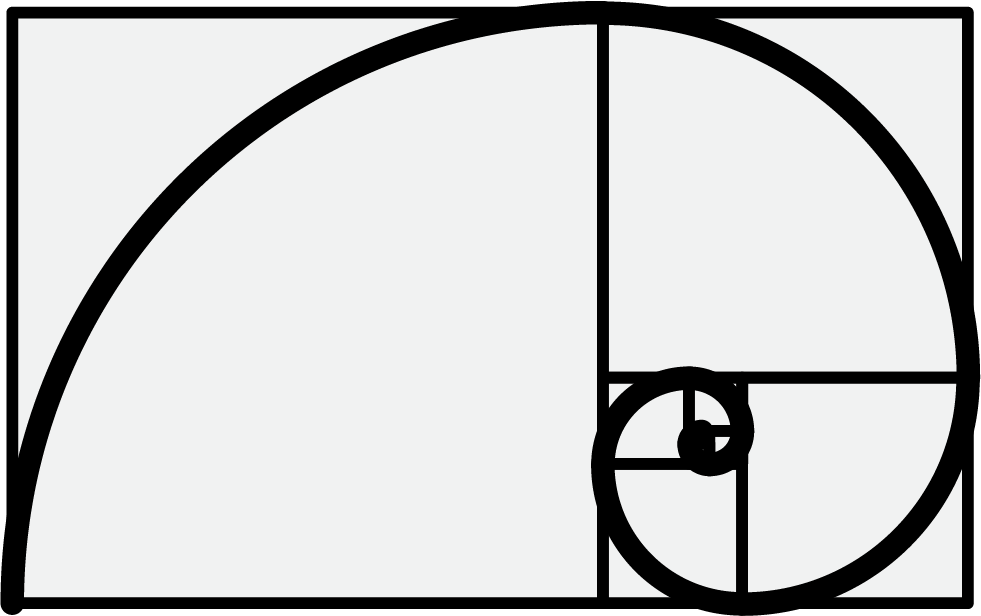
\includegraphics[height=0.75cm]{../../AAA_template_latex_settings/pwr-control_logo_doc.png}}
\lfoot{\href{https://github.com/pwr-control}{\color{black} pwr-control}}
\cfoot{-\ \thepage\ -}
\rfoot{\textit{}}
\renewcommand{\headrulewidth}{0.4pt}
\renewcommand{\footrulewidth}{0.4pt}


\geometry{
	a4paper,
	top    = 2.5cm,
	bottom = 3.0cm,
	left   = 2.5cm,
	right  = 2.5cm
}

\hypersetup{
	colorlinks = true,
	urlcolor   = blue,
	linkcolor  = black,
	citecolor  = black
}

\pagenumbering{gobble}



\usetikzlibrary{decorations.pathreplacing,fit,shapes.geometric,calc}
\usepackage[european,straightvoltages]{circuitikz}
\ctikzset{voltage dir=EF}

\newcommand{\ped}[1]{_{\mathrm{#1}}}
\newcommand{\code}[1]{\texttt{#1}}
\renewcommand{\tabularxcolumn}[1]{>{\raggedright\arraybackslash}p{#1}}
\setlength{\emergencystretch}{3em}
\sisetup{per-mode=symbol}

% ---------------- document metadata (read by the title page) ----------------
\newcommand{\DocCategory}{Technical Note}
\newcommand{\DocField}{Power Electronics and Control Systems}

\newcommand{\DocTitle}{%
	{\fontsize{20}{24}\selectfont\bfseries Active power decoupling of a single-phase AFE} \\[16pt]
	{\fontsize{16}{20}\selectfont\bfseries the ripple port and its control in the model \code{single\_phase\_afe}}
}

\newcommand{\DocSubtitle}{%
	Why the power of a single-phase converter pulsates at twice the grid frequency, how the model \code{single\_phase\_afe} of the repository \code{modelization-and-control} moves that pulsation from the DC link into a buffer capacitor through a second full bridge, and how the control loops that do it are built. With a check of the numbers of the model.
}

\newcommand{\DocAuthor}{Davide Bagnara}
\newcommand{\DocRevision}{00}
\newcommand{\DocDate}{October 2026}

\newcommand{\DocAbstract}{%
	A single-phase converter at unity power factor takes from the grid a power that pulsates at twice the grid frequency: it goes from zero to twice the average power, one hundred times per second on a \SI{50}{\hertz} grid. On a three-phase converter the three pulsations cancel; on a single-phase one they reach the DC link, where they become a voltage ripple at \SI{100}{\hertz}. The usual cure is a large DC-link capacitor. The model \code{single\_phase\_afe} does something else: a second full bridge, the \emph{ripple port}, connects a buffer capacitor to the DC link through two inductors, and a control loop makes this bridge draw from the DC link exactly the pulsating part of the power, so that the DC link sees only the average. This note explains the pulsation and the energy it moves, the circuit of the ripple port and how its parts are sized, and the control of the model step by step: the observer that isolates the ripple, the filter that builds its quadrature signal, the rotation at twice the grid angle that turns the ripple into two constants, the vector PI that drives them to zero, and the reason why the controller output is applied through the $\beta$ axis. The numbers of the model are checked with a Python script that also runs an averaged simulation of the DC-link side with the discrete loops of the model: the ripple of the DC-link voltage falls from \SI{16}{\percent} to below \SI{1}{\percent} and the third harmonic of the grid current from \SI{13}{\percent} to \SI{0.5}{\percent}. The open points found during the check are listed at the end.
}

\newcommand{\RevisionHistory}{%
	00 & October 2026 & First issue: the pulsation, the ripple port, the control chain of the model, check of the numbers, open points. & \DocAuthor \\
}

\newcommand{\MetaLabelA}{Project Repository}
\newcommand{\MetaValueAUrl}{https://github.com/pwr-control/modelization-and-control.git}
\newcommand{\MetaValueALabel}{modelization-and-control.git (foundations\_of\_power\_electronics/single\_phase\_afe)}

\newcommand{\MetaLabelB}{Framework}
\newcommand{\MetaValueB}{MATLAB/Simulink/Simscape, Python}

\begin{document}

% =============================================================
%  pwr-control LaTeX template - FRONTESPIZIO
%
%  Da richiamare come prima istruzione dopo \begin{document}:
%      % =============================================================
%  pwr-control LaTeX template - FRONTESPIZIO
%
%  Da richiamare come prima istruzione dopo \begin{document}:
%      % =============================================================
%  pwr-control LaTeX template - FRONTESPIZIO
%
%  Da richiamare come prima istruzione dopo \begin{document}:
%      \input{../../AAA_template_latex_settings/titlepage}
%
%  Il documento deve definire prima di \begin{document}:
%      \DocCategory   categoria del documento
%      \DocField      area tecnica
%      \DocTitle      titolo (una o due righe)
%      \DocSubtitle   sottotitolo
%      \DocAuthor     autore/i, separati da virgola
%      \DocRevision   numero di revisione corrente (es. 00)
%      \DocDate       data della revisione corrente
%      \DocAbstract   abstract
%      \RevisionHistory  righe della tabella di revisione, nel formato
%                        Rev. & Date & Description & Authors \\
%      \MetaLabelA \MetaValueAUrl \MetaValueALabel
%      \MetaLabelB \MetaValueB
% =============================================================

\providecommand{\DocCategory}{Technical Research Report}
\providecommand{\DocField}{Power Electronics and Control Systems}
\providecommand{\DocSubtitle}{}
\providecommand{\DocRevision}{00}
\providecommand{\DocAbstract}{}
\providecommand{\RevisionHistory}{%
	\DocRevision & \DocDate & First issue. & \DocAuthor \\
}

\titlepage

% ---- Intestazione centrata ----
\begin{center}
	{\Large\scshape \DocCategory}\\[8pt]
	{\large\scshape \DocField}
\end{center}

\vspace{30pt plus 4pt minus 14pt}
\noindent\rule{\linewidth}{0.8pt}

% ---- Titolo ----
\begin{center}
	\DocTitle
\end{center}

\vspace{4pt}
\noindent\rule{\linewidth}{2.2pt}

% ---- Sottotitolo ----
\begin{center}
	\begin{onehalfspace}
		{\large\itshape \DocSubtitle}
	\end{onehalfspace}
\end{center}

% ---- Authors / Revision / Date ----
\vspace{30pt plus 4pt minus 14pt}

\noindent
\begin{minipage}[t]{0.46\linewidth}
	\raggedright
	\textbf{Authors:}\\[2pt]
	\DocAuthor
\end{minipage}%
\hfill
\begin{minipage}[t]{0.22\linewidth}
	\centering
	\textbf{Revision:}\\[2pt]
	\DocRevision
\end{minipage}%
\hfill
\begin{minipage}[t]{0.30\linewidth}
	\raggedleft
	\textbf{Date:}\\[2pt]
	\DocDate
\end{minipage}

\vspace{10pt}
\noindent\rule{\linewidth}{0.8pt}

% ---- Abstract ----
\vspace{24pt plus 4pt minus 12pt}

\begin{center}
	\begin{minipage}{0.88\linewidth}
		\footnotesize
		\begin{onehalfspace}
			\textbf{Abstract:} \DocAbstract
		\end{onehalfspace}
	\end{minipage}
\end{center}

\vfill

% ---- Revision history ----
\begin{center}
	\begin{minipage}{0.96\linewidth}
		\centering
		{\footnotesize\scshape Revision history}\\[6pt]
		{\footnotesize
			\begin{tabular}{@{}cl>{\raggedright\arraybackslash}p{0.36\linewidth}>{\raggedright\arraybackslash}p{0.28\linewidth}@{}}
				\toprule
				\textbf{Rev.} & \textbf{Date} & \textbf{Description} & \textbf{Authors} \\
				\midrule
				\RevisionHistory
				\bottomrule
			\end{tabular}}
	\end{minipage}
\end{center}

\vspace{18pt plus 4pt minus 10pt}

% ---- Metadati in fondo ----
\noindent
\begin{tabular}{@{} r @{\quad} l @{}}
	\textsc{\MetaLabelA:} & {\href{\MetaValueAUrl}{\MetaValueALabel}} \\[3pt]
	\textsc{\MetaLabelB:} & {\MetaValueB}       \\[3pt]
\end{tabular}

% =============================================================
%  Fine frontespizio
% =============================================================
\newpage
\pagenumbering{arabic}
\setcounter{page}{1}

%
%  Il documento deve definire prima di \begin{document}:
%      \DocCategory   categoria del documento
%      \DocField      area tecnica
%      \DocTitle      titolo (una o due righe)
%      \DocSubtitle   sottotitolo
%      \DocAuthor     autore/i, separati da virgola
%      \DocRevision   numero di revisione corrente (es. 00)
%      \DocDate       data della revisione corrente
%      \DocAbstract   abstract
%      \RevisionHistory  righe della tabella di revisione, nel formato
%                        Rev. & Date & Description & Authors \\
%      \MetaLabelA \MetaValueAUrl \MetaValueALabel
%      \MetaLabelB \MetaValueB
% =============================================================

\providecommand{\DocCategory}{Technical Research Report}
\providecommand{\DocField}{Power Electronics and Control Systems}
\providecommand{\DocSubtitle}{}
\providecommand{\DocRevision}{00}
\providecommand{\DocAbstract}{}
\providecommand{\RevisionHistory}{%
	\DocRevision & \DocDate & First issue. & \DocAuthor \\
}

\titlepage

% ---- Intestazione centrata ----
\begin{center}
	{\Large\scshape \DocCategory}\\[8pt]
	{\large\scshape \DocField}
\end{center}

\vspace{30pt plus 4pt minus 14pt}
\noindent\rule{\linewidth}{0.8pt}

% ---- Titolo ----
\begin{center}
	\DocTitle
\end{center}

\vspace{4pt}
\noindent\rule{\linewidth}{2.2pt}

% ---- Sottotitolo ----
\begin{center}
	\begin{onehalfspace}
		{\large\itshape \DocSubtitle}
	\end{onehalfspace}
\end{center}

% ---- Authors / Revision / Date ----
\vspace{30pt plus 4pt minus 14pt}

\noindent
\begin{minipage}[t]{0.46\linewidth}
	\raggedright
	\textbf{Authors:}\\[2pt]
	\DocAuthor
\end{minipage}%
\hfill
\begin{minipage}[t]{0.22\linewidth}
	\centering
	\textbf{Revision:}\\[2pt]
	\DocRevision
\end{minipage}%
\hfill
\begin{minipage}[t]{0.30\linewidth}
	\raggedleft
	\textbf{Date:}\\[2pt]
	\DocDate
\end{minipage}

\vspace{10pt}
\noindent\rule{\linewidth}{0.8pt}

% ---- Abstract ----
\vspace{24pt plus 4pt minus 12pt}

\begin{center}
	\begin{minipage}{0.88\linewidth}
		\footnotesize
		\begin{onehalfspace}
			\textbf{Abstract:} \DocAbstract
		\end{onehalfspace}
	\end{minipage}
\end{center}

\vfill

% ---- Revision history ----
\begin{center}
	\begin{minipage}{0.96\linewidth}
		\centering
		{\footnotesize\scshape Revision history}\\[6pt]
		{\footnotesize
			\begin{tabular}{@{}cl>{\raggedright\arraybackslash}p{0.36\linewidth}>{\raggedright\arraybackslash}p{0.28\linewidth}@{}}
				\toprule
				\textbf{Rev.} & \textbf{Date} & \textbf{Description} & \textbf{Authors} \\
				\midrule
				\RevisionHistory
				\bottomrule
			\end{tabular}}
	\end{minipage}
\end{center}

\vspace{18pt plus 4pt minus 10pt}

% ---- Metadati in fondo ----
\noindent
\begin{tabular}{@{} r @{\quad} l @{}}
	\textsc{\MetaLabelA:} & {\href{\MetaValueAUrl}{\MetaValueALabel}} \\[3pt]
	\textsc{\MetaLabelB:} & {\MetaValueB}       \\[3pt]
\end{tabular}

% =============================================================
%  Fine frontespizio
% =============================================================
\newpage
\pagenumbering{arabic}
\setcounter{page}{1}

%
%  Il documento deve definire prima di \begin{document}:
%      \DocCategory   categoria del documento
%      \DocField      area tecnica
%      \DocTitle      titolo (una o due righe)
%      \DocSubtitle   sottotitolo
%      \DocAuthor     autore/i, separati da virgola
%      \DocRevision   numero di revisione corrente (es. 00)
%      \DocDate       data della revisione corrente
%      \DocAbstract   abstract
%      \RevisionHistory  righe della tabella di revisione, nel formato
%                        Rev. & Date & Description & Authors \\
%      \MetaLabelA \MetaValueAUrl \MetaValueALabel
%      \MetaLabelB \MetaValueB
% =============================================================

\providecommand{\DocCategory}{Technical Research Report}
\providecommand{\DocField}{Power Electronics and Control Systems}
\providecommand{\DocSubtitle}{}
\providecommand{\DocRevision}{00}
\providecommand{\DocAbstract}{}
\providecommand{\RevisionHistory}{%
	\DocRevision & \DocDate & First issue. & \DocAuthor \\
}

\titlepage

% ---- Intestazione centrata ----
\begin{center}
	{\Large\scshape \DocCategory}\\[8pt]
	{\large\scshape \DocField}
\end{center}

\vspace{30pt plus 4pt minus 14pt}
\noindent\rule{\linewidth}{0.8pt}

% ---- Titolo ----
\begin{center}
	\DocTitle
\end{center}

\vspace{4pt}
\noindent\rule{\linewidth}{2.2pt}

% ---- Sottotitolo ----
\begin{center}
	\begin{onehalfspace}
		{\large\itshape \DocSubtitle}
	\end{onehalfspace}
\end{center}

% ---- Authors / Revision / Date ----
\vspace{30pt plus 4pt minus 14pt}

\noindent
\begin{minipage}[t]{0.46\linewidth}
	\raggedright
	\textbf{Authors:}\\[2pt]
	\DocAuthor
\end{minipage}%
\hfill
\begin{minipage}[t]{0.22\linewidth}
	\centering
	\textbf{Revision:}\\[2pt]
	\DocRevision
\end{minipage}%
\hfill
\begin{minipage}[t]{0.30\linewidth}
	\raggedleft
	\textbf{Date:}\\[2pt]
	\DocDate
\end{minipage}

\vspace{10pt}
\noindent\rule{\linewidth}{0.8pt}

% ---- Abstract ----
\vspace{24pt plus 4pt minus 12pt}

\begin{center}
	\begin{minipage}{0.88\linewidth}
		\footnotesize
		\begin{onehalfspace}
			\textbf{Abstract:} \DocAbstract
		\end{onehalfspace}
	\end{minipage}
\end{center}

\vfill

% ---- Revision history ----
\begin{center}
	\begin{minipage}{0.96\linewidth}
		\centering
		{\footnotesize\scshape Revision history}\\[6pt]
		{\footnotesize
			\begin{tabular}{@{}cl>{\raggedright\arraybackslash}p{0.36\linewidth}>{\raggedright\arraybackslash}p{0.28\linewidth}@{}}
				\toprule
				\textbf{Rev.} & \textbf{Date} & \textbf{Description} & \textbf{Authors} \\
				\midrule
				\RevisionHistory
				\bottomrule
			\end{tabular}}
	\end{minipage}
\end{center}

\vspace{18pt plus 4pt minus 10pt}

% ---- Metadati in fondo ----
\noindent
\begin{tabular}{@{} r @{\quad} l @{}}
	\textsc{\MetaLabelA:} & {\href{\MetaValueAUrl}{\MetaValueALabel}} \\[3pt]
	\textsc{\MetaLabelB:} & {\MetaValueB}       \\[3pt]
\end{tabular}

% =============================================================
%  Fine frontespizio
% =============================================================
\newpage
\pagenumbering{arabic}
\setcounter{page}{1}


\tableofcontents
\listoffigures
\listoftables
\newpage

\begin{onehalfspace}

% =============================================================
\section*{Nomenclature}
\addcontentsline{toc}{section}{Nomenclature}
\label{sec:nomenclature}

\rowcolors{2}{tableShade}{white}
\begin{longtable}{@{} l p{0.74\linewidth} @{}}
	\toprule
	\textbf{Symbol} & \textbf{Meaning} \\
	\midrule
	\endfirsthead
	\toprule
	\textbf{Symbol} & \textbf{Meaning} \\
	\midrule
	\endhead
	\bottomrule
	\endfoot
	\bottomrule
	\endlastfoot
	AFE & active front end: a PWM converter between a DC link and the AC grid, power in both directions \\
	APD & active power decoupling: removing the power pulsation from the DC link with a controlled circuit instead of a large capacitor \\
	ripple port & the second full bridge of the model, with the buffer capacitor on its DC side and its AC side tied to the DC link through two inductors \\
	pu & per unit: a quantity divided by its base value \\
	$U$, $I$ & peak values of the grid voltage and of the grid current (fundamental) \\
	$P$, $S$ & average active power and apparent power of the single-phase connection \\
	$\omega$, $f$ & angular frequency $2\pi f$ and frequency of the grid (\SI{50}{\hertz}); the pulsation is at $2\omega$ (\SI{100}{\hertz}) \\
	$\theta$ & grid angle from the PLL; the ripple loop uses $2\theta$ \\
	$u\ped{dc}$, $u\ped{dc,nom}$ & DC-link voltage and its base (\SI{1239.4}{\volt}); $u\ped{dc,pu} = u\ped{dc}/u\ped{dc,nom}$ \\
	$C\ped{dc}$ & DC-link capacitor (\SI{2.4}{\milli\farad}) \\
	$u\ped{b}$, $C\ped{b}$, $L\ped{b}$ & buffer voltage, buffer capacitor (\SI{3.6}{\milli\farad}) and the two inductors of the ripple port (\SI{250}{\micro\henry} each) \\
	$i\ped{b}$ & current from the DC link into the ripple port (positive when the buffer takes energy) \\
	$i\ped{b,bez}$ & base of the buffer current acquisition (\SI{750}{\ampere}) \\
	$m\ped{b}$ & duty (modulation index) of the ripple-port bridge, $u\ped{dc} \approx m\ped{b}\, u\ped{b}$ on average \\
	$u\ped{bez}$, $i\ped{bez}$ & bases of the grid-side quantities of the model (\SI{838.4}{\volt}, \SI{536.8}{\ampere}) \\
	$t\ped{s}$ & control period, \SI{100}{\micro\second} (\SI{5}{\kilo\hertz} PWM, double update) \\
	$\alpha\beta$, $dq$ & stationary and rotating two-axis frames; in the ripple loop the frame turns at $2\theta$ \\
	FHT & first harmonic tracker: a resonant observer that extracts the fundamental of a signal and its quadrature \\
	PI, vector PI & proportional-integral controller; the vector PI is a PI on the $d$ and $q$ components with one common output limit \\
	$k\ped{p}$, $k\ped{i}$ & proportional and integral gains, output in pu per pu of error; $k\ped{i}$ in \si{\per\second} \\
\end{longtable}
\addtocounter{table}{-1}
\rowcolors{1}{white}{white}

% =============================================================
\section{Introduction}
\label{sec:intro}

A converter connected to one phase of the grid has a problem that a three-phase converter does not have: the power it exchanges with the grid is not constant. With a sinusoidal voltage and a sinusoidal current in phase, the instantaneous power is the product of two sinusoids at the same frequency, which is a constant plus a cosine at twice the frequency. The power goes from zero to twice its average value and back, one hundred times per second on a \SI{50}{\hertz} grid. The DC side of the converter has to take this pulsation. On a three-phase converter the three phases pulsate with \SI{120}{\degree} between them and the sum is constant; on a single-phase converter there is nothing to cancel it.

The pulsating power has to be stored somewhere. The simplest place is the DC-link capacitor: the energy that comes in during one quarter of the grid period goes out during the next, and the DC-link voltage goes up and down at \SI{100}{\hertz}. To keep the ripple small the capacitor has to be large, and in a \SI{225}{\kilo\watt} converter at \SI{1200}{\volt} ``large'' means tens of millifarads of electrolytic capacitors. The alternative is \emph{active power decoupling} (APD): a small extra circuit with its own energy storage takes the pulsating part of the power, and the DC link sees only the average. The storage element can then work with a large voltage swing, which means much less capacitance for the same energy \cite{krein2012,sun2016,hu2013}.

The model \code{single\_phase\_afe} of the repository \code{modelization-and-control} is a single-phase full-bridge AFE between two phases of a \SI{690}{\volt} grid with such a circuit: a second full bridge, called here the \emph{ripple port}, with a buffer capacitor on its DC side and its AC side tied to the DC link through two inductors. A control loop makes the ripple port draw from the DC link a current at \SI{100}{\hertz} that is exactly the pulsating part of the power divided by the DC-link voltage. This note describes how.

Section~\ref{sec:pulsation} gives the pulsation and the energy that moves. Section~\ref{sec:circuit} is the circuit of the model and the sizing of its parts. Section~\ref{sec:control} is the control, loop by loop, with the reason of each block. Section~\ref{sec:results} shows what the decoupling does with an averaged simulation and Section~\ref{sec:check} checks the numbers of the model. Section~\ref{sec:open} lists the open points. Everything is in simple words; the equations are the few that one needs to size the parts and to set the gains.

% =============================================================
\section{The power pulsation of a single-phase converter}
\label{sec:pulsation}

\subsection{The instantaneous power}

Take the grid voltage and the grid current as
\begin{equation}
	u(t) = U \cos(\omega t), \qquad i(t) = I \cos(\omega t - \varphi),
\end{equation}
with $U$ and $I$ the peak values and $\varphi$ the phase of the current behind the voltage. The instantaneous power is
\begin{equation}
	p(t) = u(t)\, i(t) = \frac{U I}{2} \cos\varphi + \frac{U I}{2} \cos(2\omega t - \varphi) = P + S \cos(2\omega t - \varphi),
	\label{eq:power}
\end{equation}
where $P = (UI/2)\cos\varphi$ is the average (active) power and $S = UI/2$ is the apparent power. The second term pulsates at $2\omega$ with amplitude $S$: at unity power factor it is as large as the active power, and it does not become smaller when the current is reactive. At unity power factor ($\varphi = 0$):
\begin{equation}
	p(t) = P\,\big(1 + \cos 2\omega t\big).
\end{equation}
Figure~\ref{fig:pulsation} shows it with the numbers of the model: \SI{225}{\kilo\watt} average, \SI{450}{\kilo\watt} peak, zero at the zero crossings of voltage and current.

\begin{figure}[H]
	\centering
	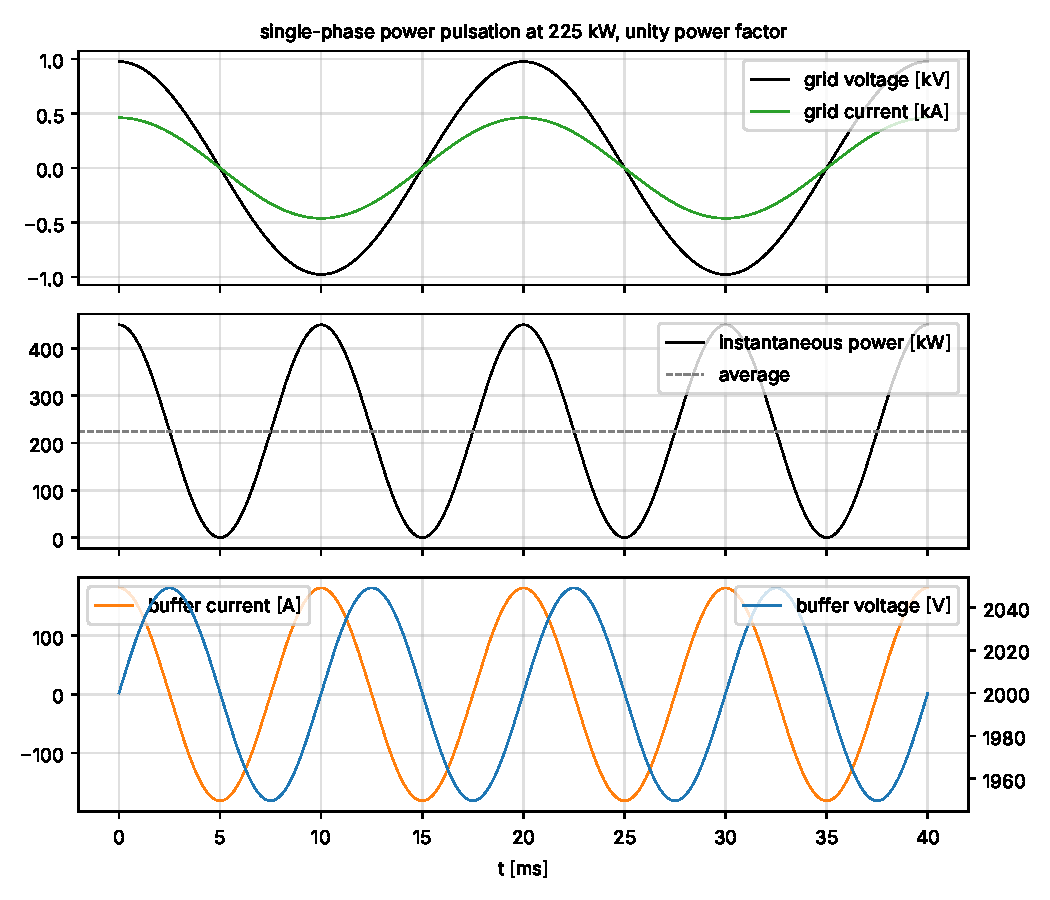
\includegraphics[width=0.78\linewidth]{figures/single_phase_afe_power_pulsation.pdf}
	\captionsetup{width=0.9\textwidth, font=small}
	\caption[The power pulsation at \SI{225}{\kilo\watt}.]{The power pulsation of the model at \SI{225}{\kilo\watt} and unity power factor: grid voltage and current (top), instantaneous power (middle), and the current and the voltage of an ideal buffer of \SI{3.6}{\milli\farad} at \SI{2000}{\volt} that takes the whole pulsation (bottom). Figure of \code{single\_phase\_afe\_design\_check.py}.}
	\label{fig:pulsation}
\end{figure}

\subsection{The energy that moves}

The pulsating part of the power, $P\cos 2\omega t$, is the rate at which energy enters and leaves the storage. Its integral is the energy stored:
\begin{equation}
	e(t) = \int P \cos(2\omega t)\, dt = \frac{P}{2\omega} \sin(2\omega t),
	\qquad \Delta E = e\ped{max} - e\ped{min} = \frac{P}{\omega}.
	\label{eq:energy}
\end{equation}
This is the number that sizes any storage element, passive or active: at \SI{225}{\kilo\watt} and \SI{50}{\hertz}, $\Delta E = 225\,000/314.16 = \SI{716}{\joule}$ peak-to-peak (\SI{875}{\joule} at the \SI{275}{\kilo\watt} load of the model).

\subsection{What the DC link alone would do}

If the DC-link capacitor $C\ped{dc}$ takes the whole pulsation, the current that enters it at $2\omega$ has amplitude $P/u\ped{dc}$ and the voltage ripple has amplitude
\begin{equation}
	\Delta u\ped{dc} = \frac{P}{2\omega\, C\ped{dc}\, u\ped{dc}}.
	\label{eq:ripple}
\end{equation}
With $C\ped{dc} = \SI{2.4}{\milli\farad}$ and $u\ped{dc} = \SI{1239}{\volt}$ this is \SI{120}{\volt} (\SI{9.7}{\percent}) at \SI{225}{\kilo\watt} and \SI{147}{\volt} (\SI{11.9}{\percent}) at \SI{275}{\kilo\watt}, with an rms current of \SI{128}{\ampere} in the capacitor. A ripple of \SI{1}{\percent} would need \SI{23}{\milli\farad}. The ripple is not only a stress for the capacitor: Section~\ref{sec:results} shows that it also goes through the DC-link voltage controller into the grid current reference and distorts the grid current.

Energy in a capacitor goes with the square of the voltage. A capacitor that swings between $u\ped{min}$ and $u\ped{max}$ stores
\begin{equation}
	\Delta E = \frac{C}{2}\left(u\ped{max}^2 - u\ped{min}^2\right),
	\label{eq:cap_energy}
\end{equation}
so for the same $\Delta E$ a capacitor that is allowed to swing by $\pm\SI{5}{\percent}$ around \SI{2000}{\volt} needs only $716 / (0.5 \cdot (2100^2 - 1900^2)) = \SI{1.79}{\milli\farad}$. This is why the buffer of an active decoupling circuit can be small: it is not asked to keep its voltage constant.

% =============================================================
\section{The ripple port of the model}
\label{sec:circuit}

\subsection{Circuit}

Figure~\ref{fig:circuit} is the power circuit of \code{single\_phase\_afe}. From left to right:

\begin{itemize}[nosep]
	\item the grid: the three-phase emulator of the library gives the phase voltages of a \SI{690}{\volt}, \SI{50}{\hertz} grid; the converter is connected between phases $a$ and $b$, so it sees the line-to-line voltage $u\ped{ab}$, \SI{975.8}{\volt} peak;
	\item the LCL filter: $L_2 = \SI{250}{\micro\henry}$ on the grid side, $C\ped{f} = \SI{200}{\micro\farad}$ with \SI{50}{\milli\ohm} in series, $L_1 = \SI{250}{\micro\henry}$ on the converter side; resonance at \SI{1007}{\hertz};
	\item the AFE: a full bridge of four IGBTs with antiparallel diodes (Infineon FF1200R17IP5, \SI{1700}{\volt}, one half-bridge module per leg), unipolar PWM at \SI{5}{\kilo\hertz};
	\item the DC link: $C\ped{dc} = \SI{2.4}{\milli\farad}$, nominal voltage $u\ped{dc,nom} = \SI{1239.4}{\volt}$, and the load, a current source that ramps to \SI{275}{\kilo\watt} in \SI{0.25}{\second};
	\item the ripple port: a second full bridge, same module, whose two leg midpoints are tied to the two rails of the DC link through $L\ped{b} = \SI{250}{\micro\henry}$ each (\SI{4}{\milli\ohm}), and whose DC side is the buffer capacitor $C\ped{b} = \SI{3.6}{\milli\farad}$ kept at \SI{2000}{\volt}.
\end{itemize}

\begin{figure}[H]
	\centering
	\ctikzset{transistors/scale=0.7, bipoles/length=0.9cm}
	\begin{circuitikz}[european, font=\scriptsize, scale=0.8, transform shape]
		% ---- grid and LCL filter
		\draw (0,0.6) to[sV, l=$u\ped{ab}$] (0,2.4) to[L, l=$L_2$] (1.7,2.4) -- (2.5,2.4) to[L, l=$L_1$] (4.2,2.4) -- (6.0,2.4);
		\draw (2.5,2.4) to[R, l_=\SI{50}{\milli\ohm}] (2.5,1.5) to[C, l_=$C\ped{f}$] (2.5,0.6);
		\draw (0,0.6) -- (7.6,0.6);
		\fill (2.5,2.4) circle (1.2pt); \fill (2.5,0.6) circle (1.2pt);
		% ---- AFE full bridge: leg a (x=6.0, midpoint y=2.4), leg b (x=7.6, midpoint y=0.6); rails y=4 and y=-1
		\draw (5.4,4) -- (11.9,4) node[midway, above] {};
		\draw (5.4,-1) -- (11.9,-1);
		\draw (6.0,4) to[Tnigbt] (6.0,2.4) to[Tnigbt] (6.0,-1);
		\draw (6.7,2.4) to[D] (6.7,4);  \draw (6.7,-1) to[D] (6.7,2.4);
		\draw (7.6,4) to[Tnigbt] (7.6,0.6) to[Tnigbt] (7.6,-1);
		\draw (8.3,0.6) to[D] (8.3,4);  \draw (8.3,-1) to[D] (8.3,0.6);
		\foreach \p in {(6.0,4),(6.0,2.4),(6.0,-1),(6.7,4),(6.7,2.4),(6.7,-1),(7.6,4),(7.6,0.6),(7.6,-1),(8.3,4),(8.3,0.6),(8.3,-1)} {\fill \p circle (1.2pt);}
		\node[above, font=\scriptsize\bfseries] at (7.0,4.05) {AFE};
		% ---- DC link and load
		\draw (9.4,4) to[C, l=$C\ped{dc}$, v=$u\ped{dc}$] (9.4,-1);
		\draw (10.8,4) to[I, l=$i\ped{load}$] (10.8,-1);
		\foreach \p in {(9.4,4),(9.4,-1),(10.8,4),(10.8,-1),(11.9,4),(11.9,-1)} {\fill \p circle (1.2pt);}
		% ---- ripple port: inductors from the rails to the leg midpoints c (y=4) and d (y=-1)
		\draw (11.9,4) to[L, l=$L\ped{b}$, i=$i\ped{b}$] (13.6,4);
		\draw (11.9,-1) to[L, l_=$L\ped{b}$] (13.6,-1);
		\draw (13.0,5.2) -- (17.6,5.2);
		\draw (13.0,-2.2) -- (17.6,-2.2);
		\draw (13.6,5.2) to[Tnigbt] (13.6,4) to[Tnigbt] (13.6,-2.2);
		\draw (14.3,4) to[D] (14.3,5.2);  \draw (14.3,-2.2) to[D] (14.3,4);
		\draw (15.2,5.2) to[Tnigbt] (15.2,-1) to[Tnigbt] (15.2,-2.2);
		\draw (15.9,-1) to[D] (15.9,5.2);  \draw (15.9,-2.2) to[D] (15.9,-1);
		\draw (17.0,5.2) to[C, l=$C\ped{b}$, v=$u\ped{b}$] (17.0,-2.2);
		\foreach \p in {(13.6,5.2),(13.6,4),(13.6,-2.2),(14.3,5.2),(14.3,4),(14.3,-2.2),(15.2,5.2),(15.2,-1),(15.2,-2.2),(15.9,5.2),(15.9,-1),(15.9,-2.2),(17.0,5.2),(17.0,-2.2)} {\fill \p circle (1.2pt);}
		\node[above, font=\scriptsize\bfseries] at (14.8,5.25) {ripple port};
	\end{circuitikz}
	\captionsetup{width=0.92\textwidth, font=small}
	\caption[Power circuit of the model.]{Power circuit of \code{single\_phase\_afe}: grid voltage $u\ped{ab}$, LCL filter, AFE full bridge, DC link with the current-source load, and the ripple port: a second full bridge whose leg midpoints reach the DC-link rails through the two inductors $L\ped{b}$ and whose DC side is the buffer capacitor $C\ped{b}$. Both bridges are drawn with their antiparallel diodes.}
	\label{fig:circuit}
\end{figure}

\subsection{How the ripple port works}

Seen from the buffer, the ripple port is a full-bridge DC-DC converter whose ``output'' is the DC link: with the duty $m\ped{b}$ it applies to the inductors a voltage whose average is $m\ped{b} u\ped{b}$, and the current $i\ped{b}$ in the inductors obeys
\begin{equation}
	L\ped{b,tot}\, \frac{d i\ped{b}}{dt} = u\ped{dc} - m\ped{b}\, u\ped{b} - R\ped{b}\, i\ped{b}, \qquad L\ped{b,tot} = 2 L\ped{b} = \SI{500}{\micro\henry},
	\label{eq:ib}
\end{equation}
where $i\ped{b}$ is counted from the DC link into the port (positive when the buffer takes energy). Note the sign: a larger duty makes the current \emph{smaller}. This is a boost stage seen from the DC link, so the buffer voltage must always stay above $u\ped{dc}$: in the model $u\ped{b} = \SI{2000}{\volt}$ against $u\ped{dc} = \SI{1239}{\volt}$, and the steady duty is $m\ped{b} = u\ped{dc}/u\ped{b} = 0.62$. The buffer gets the charge $m\ped{b} i\ped{b}$:
\begin{equation}
	C\ped{b}\, \frac{d u\ped{b}}{dt} = m\ped{b}\, i\ped{b}.
	\label{eq:ub}
\end{equation}

To decouple the pulsation, the port has to take from the DC link the pulsating part of the power. The current that does it is
\begin{equation}
	i\ped{b}^*(t) = \frac{P}{u\ped{dc}} \cos(2\omega t) \quad (\text{\SI{182}{\ampere} peak at \SI{225}{\kilo\watt}, \SI{222}{\ampere} at \SI{275}{\kilo\watt}}),
	\label{eq:ib_ref}
\end{equation}
plus a small DC component that covers the losses of the port and keeps the buffer at its reference. With this current the net current into $C\ped{dc}$ has no \SI{100}{\hertz} term and $u\ped{dc}$ is flat (Figure~\ref{fig:pulsation}, bottom: the buffer takes the energy, its voltage swings from \SI{1950}{\volt} to \SI{2049}{\volt}, and the DC link does not see it).

\subsection{Sizing}

\begin{description}[nosep, leftmargin=1.5em]
	\item[Buffer capacitor.] From \eqref{eq:energy} and \eqref{eq:cap_energy}: $C\ped{b} = 2\Delta E / (u\ped{max}^2 - u\ped{min}^2)$. The model has \SI{3.6}{\milli\farad} (half of the \SI{7.2}{\milli\farad} of the legacy data set) at \SI{2000}{\volt}: \SI{716}{\joule} give a swing of $\pm\SI{2.5}{\percent}$ (\SIrange{1950}{2049}{\volt}); the capacitor is oversized by a factor of two for a $\pm\SI{5}{\percent}$ swing (\SI{1.79}{\milli\farad}), or it could work at \SI{1500}{\volt} with \SI{3.18}{\milli\farad}.
	\item[Buffer voltage.] It must stay above $u\ped{dc}$ at the bottom of the swing, with a margin for the inductor voltage and for transients; \SI{2000}{\volt} does that with a wide margin, but it is above the \SI{1700}{\volt} class of the module (\SI{118}{\percent} of the blocking voltage): see Section~\ref{sec:open}.
	\item[Inductors.] They carry the \SI{100}{\hertz} current and filter the switching ripple. At \SI{100}{\hertz}, \SI{500}{\micro\henry} drop only \SI{57}{\volt} at \SI{182}{\ampere}, so the current loop needs little voltage. The worst-case switching ripple of a unipolar full bridge at \SI{5}{\kilo\hertz} (effective \SI{10}{\kilo\hertz}) is $u\ped{b}/(8 L\ped{b,tot} \cdot 2 f\ped{pwm}) \approx \SI{100}{\ampere}$ peak-to-peak.
	\item[Bridge.] The current is \SI{182}{\ampere} peak, \SI{0.24}{pu} of the acquisition base of \SI{750}{\ampere}; the module is the same \SI{1200}{\ampere} one of the AFE, far from its current limit, chosen for the voltage.
	\item[Current base.] The buffer current is measured with a base of \SI{750}{\ampere} (\code{param.afe.buffer.ibez}); the buffer voltage with the DC-link base $u\ped{dc,nom}$, so its reference is $2000/1239.4 = \SI{1.614}{pu}$.
\end{description}

Table~\ref{tab:numbers} collects the numbers.

\begin{table}[H]
	\centering
	\captionsetup{width=0.9\textwidth, font=small}
	\caption[Numbers of the model.]{Numbers of the model (\code{init\_model.m}) and derived figures.}
	\label{tab:numbers}
	\rowcolors{2}{tableShade}{white}
	\begin{tabularx}{0.97\textwidth}{@{} l l X @{}}
		\toprule
		\textbf{Quantity} & \textbf{Value} & \textbf{Note} \\
		\midrule
		grid & \SI{690}{\volt}, \SI{50}{\hertz} & line-to-line $a$--$b$, \SI{975.8}{\volt} peak = \SI{1.164}{pu} of $u\ped{bez}$ \\
		rating / load & \SI{225}{\kilo\watt} / \SI{275}{\kilo\watt} & \SI{461}{\ampere} / \SI{564}{\ampere} peak; the load is \SI{122}{\percent} of the rating \\
		PWM, control & \SI{5}{\kilo\hertz}, $t\ped{s} = \SI{100}{\micro\second}$ & unipolar, double update; dead time \SI{1}{\micro\second} \\
		bases & \SI{838.4}{\volt}, \SI{536.8}{\ampere}, \SI{1239.4}{\volt} & $u\ped{bez}$, $i\ped{bez}$, $u\ped{dc,nom}$ of the legacy single-phase data set \\
		LCL & \SI{250}{\micro\henry}, \SI{200}{\micro\farad}, \SI{250}{\micro\henry} & $f\ped{res} = \SI{1007}{\hertz}$, $f\ped{s}/6 = \SI{1667}{\hertz}$; $C\ped{f}$ takes \SI{13}{\percent} of $P$ as reactive power \\
		modulation index & 0.79 & at \SI{225}{\kilo\watt}, limit 1 \\
		DC link & \SI{2.4}{\milli\farad} & ripple alone \SI{9.7}{\percent} at \SI{225}{\kilo\watt}, \SI{11.9}{\percent} at \SI{275}{\kilo\watt} \\
		pulsation & \SI{182}{\ampere}, \SI{716}{\joule} & \SI{100}{\hertz} current amplitude and energy peak-to-peak at \SI{225}{\kilo\watt} \\
		buffer & \SI{3.6}{\milli\farad}, \SI{2000}{\volt} & \SI{7200}{\joule} stored, swing \SIrange{1950}{2049}{\volt} (\SI{5}{\percent}) \\
		port inductors & $2 \times \SI{250}{\micro\henry}$, \SI{4}{\milli\ohm} & \SI{57}{\volt} at \SI{100}{\hertz}, switching ripple \SI{100}{\ampere} pk-pk \\
		port duty & 0.62 & $u\ped{dc}/u\ped{b}$; the feed-forward of the current loop uses $u\ped{dc,pu} \approx 1$ instead \\
		module & FF1200R17IP5 & \SI{1700}{\volt}, \SI{1200}{\ampere}; $t\ped{d,off} + t\ped{f} = \SI{1.74}{\micro\second}$ at \SI{125}{\celsius} \\
		\bottomrule
	\end{tabularx}
	\rowcolors{1}{white}{white}
\end{table}

% =============================================================
\section{The control of the model}
\label{sec:control}

\subsection{Overview}

Figure~\ref{fig:control} shows the whole control. Everything runs at $t\ped{s} = \SI{100}{\micro\second}$, triggered at the bottom and at the top of the \SI{5}{\kilo\hertz} carrier. The grid side is a standard grid-following AFE: a PLL gives the grid angle $\theta$, a PI on the DC-link voltage gives the amplitude of the grid current, and a current loop makes the current follow a sinusoid in phase with the grid voltage. The ripple port has three loops: a slow PI on the buffer voltage that sets the DC component of the port current, the \emph{ripple loop} that sets its \SI{100}{\hertz} component, and a fast PI on the port current that applies the sum through the duty of the ripple-port bridge.

\begin{figure}[H]
	\centering
	\begin{tikzpicture}[font=\scriptsize, >=Latex, node distance=0.45cm and 0.55cm,
		blk/.style={draw, thick, rounded corners=2pt, minimum height=0.8cm, minimum width=1.7cm, align=center, fill=orange!15},
		meas/.style={draw, thick, rounded corners=2pt, minimum height=0.8cm, align=center, fill=gray!12},
		sum/.style={draw, circle, thick, inner sep=1pt, minimum size=0.45cm}]
		% ---- grid side
		\node[meas] (pll) {FHT-PLL\\grid voltages};
		\node[blk, right=of pll] (udc) {DC-link voltage PI\\$k\ped{p}\,2$, $k\ped{i}\,35$, $\pm 1.65$};
		\node[blk, right=of udc] (cc) {grid current loop\\FHT virtual $\beta$, $dq$ at $\theta$\\vector PI $0.5/45$, limit 1};
		\node[blk, right=of cc] (pwm1) {unipolar PWM\\AFE bridge};
		\draw[->] (pll) -- (udc) node[midway, above] {$\theta$};
		\draw[->] (udc) -- (cc) node[midway, above] {$I^*$};
		\draw[->] (cc) -- (pwm1) node[midway, above] {$m$};
		\node[above=0.15cm of udc.north west, anchor=south west, font=\small\bfseries] {grid side};
		% ---- ripple port
		\node[blk, below=1.5cm of pll.south west, anchor=north west] (ub) {buffer voltage PI\\$k\ped{p}\,2$, $k\ped{i}\,18$, $\pm 1$\\ref.\ \SI{2000}{\volt}, \SI{20}{\milli\second} filter};
		\node[blk, below=0.5cm of ub, fill=blue!10] (apd) {ripple loop (Figure~\ref{fig:ripple_loop})\\observer, quadrature, $dq$ at $2\theta$\\vector PI $1/18$, limit 1, on at \SI{0.5}{\second}};
		\node[sum, right=1.0cm of ub.east |- apd.north east, yshift=-0.0cm] (s) {$+$};
		\node[blk, right=of s] (ic) {buffer current PI\\$k\ped{p}\,1$, $k\ped{i}\,18$, $\pm 1$\\feed-forward $u\ped{dc,pu}$};
		\node[blk, right=of ic] (pwm2) {unipolar PWM\\ripple-port bridge};
		\draw[->] (ub.east) -| (s.north) node[pos=0.2, above] {$i\ped{b,dc}^*$};
		\draw[->] (apd.east) -| (s.south) node[pos=0.2, below] {$i\ped{b,ac}^*$};
		\draw[->] (s) -- (ic) node[midway, above] {$i\ped{b}^*$};
		\draw[->] (ic) -- (pwm2) node[midway, above] {$m\ped{b}$};
		\node[above=0.15cm of ub.north west, anchor=south west, font=\small\bfseries] {ripple port};
		% ---- measurements
		\node[meas, left=0.6cm of ub, align=center] (m1) {$u\ped{b}$};
		\node[meas, left=0.6cm of apd] (m2) {$u\ped{dc,pu}$, $2\theta$};
		\draw[->] (m1) -- (ub); \draw[->] (m2) -- (apd);
	\end{tikzpicture}
	\captionsetup{width=0.92\textwidth, font=small}
	\caption[Control of the model.]{Control of \code{single\_phase\_afe}. Grid side: PLL, DC-link voltage loop, grid current loop and PWM of the AFE. Ripple port: the buffer voltage PI gives the DC part of the port current reference, the ripple loop its \SI{100}{\hertz} part, and the buffer current PI applies the sum through the duty of the ripple-port bridge. Gains in pu per pu; $k\ped{i}$ in \si{\per\second}.}
	\label{fig:control}
\end{figure}

\subsection{Grid side}

\begin{description}[nosep, leftmargin=1.5em]
	\item[PLL.] A first harmonic tracker on each of the three grid voltages, Clarke transform, positive sequence, and a phase observer (\code{pll\_stageB}: PI $k\ped{p}\,1$, $k\ped{i}\,80$ on the $q$ voltage, double-integrator observer of angle and frequency). The angle $\theta$ is the angle of the line-to-line voltage $u\ped{ab}$ seen by the converter; the ripple loop uses $2\theta$.
	\item[DC-link voltage loop.] The reference is \SI{1}{pu}, applied as a step at \SI{1}{\milli\second} through a \SI{20}{\milli\second} low-pass. The PI ($k\ped{p}\,2$, $k\ped{i}\,35$, output between $\pm\SI{1.65}{pu}$, with anti-windup) gives the amplitude of the grid current $I^*$, negative when the converter rectifies. The plant is the DC-link capacitor through the power balance: \SI{1}{pu} of current amplitude changes $u\ped{dc,pu}$ by \SI{71}{\per\second}; the crossover is \SI{23}{\hertz} with \SI{79}{\degree} of phase margin. The PI has no filter at \SI{100}{\hertz}: $|k\ped{p} + k\ped{i}/(j 2\omega)| = 2.0$, so a ripple of \SI{10}{\percent} on $u\ped{dc,pu}$ becomes \SI{0.2}{pu} of \SI{100}{\hertz} on the current amplitude. This matters when the ripple loop is off (Section~\ref{sec:results}).
	\item[Grid current loop.] The measured current is the $\alpha$ component; a first harmonic tracker (a resonant observer at $\omega$ with damping $\delta = 0.05$ and observer poles at $-\omega$ and $-4\omega$) gives the fundamental and its quadrature, which is the virtual $\beta$. After the rotation at $\theta$ the current is a $dq$ vector; the reference is $d = I^*$, $q = 0$ (unity power factor). The vector PI ($k\ped{p}\,0.5$, $k\ped{i}\,45$, output divided by $u\ped{dc,pu}$ and limited to 1 as a vector, with the integrators frozen while the limit is active) gives the voltage reference, rotated back to $\alpha\beta$; the $\alpha$ component is the modulation index of the AFE bridge. With the LCL the crossover is \SI{325}{\hertz} with \SI{70}{\degree} of phase margin; the resonance of the filter at \SI{1007}{\hertz} is below $f\ped{s}/6$, the region where the converter-side current feedback damps it by itself, and the \SI{50}{\milli\ohm} of the capacitor branch help; the gain margin at the resonance is \SI{5}{\decibel}.
\end{description}

\subsection{The ripple loop, step by step}
\label{sec:ripple_loop}

The ripple loop is the part that does the decoupling (Figure~\ref{fig:ripple_loop}). It has to find the \SI{100}{\hertz} ripple of the DC-link voltage, measure its amplitude and its phase, and ask the ripple port for the current that cancels it. The model does it with the same tools used for the grid current: a quadrature pair, a rotation into a frame that turns with the ripple, and a vector PI on the two constants that come out.

\begin{figure}[H]
	\centering
	\begin{tikzpicture}[font=\scriptsize, >=Latex, node distance=0.4cm and 0.5cm,
		blk/.style={draw, thick, rounded corners=2pt, minimum height=0.95cm, minimum width=1.5cm, align=center, fill=blue!10},
		sm/.style={draw, thick, rounded corners=2pt, minimum height=0.6cm, align=center, fill=gray!12}]
		\node[sm] (in) {$u\ped{dc,pu}$};
		\node[blk, right=of in] (obs) {double-integrator\\observer\\$\hat v / \omega$};
		\node[blk, right=of obs] (ps) {phase-shift filter\\$(z-a)/(z-b)$ at $2f$\\$\times(-1)$};
		\node[blk, right=of ps] (park) {$\alpha\beta \to dq$\\at $2\theta$};
		\node[blk, right=of park] (pi) {vector PI\\$k\ped{p}\,1$, $k\ped{i}\,18$\\ref.\ $0$, limit 1};
		\node[blk, right=of pi] (ipark) {$dq \to \alpha\beta$\\at $2\theta$\\\textbf{$\beta$ output}};
		\node[sm, right=of ipark] (out) {$i\ped{b,ac}^*$};
		\draw[->] (in) -- (obs);
		\draw[->] (obs) -- (ps) node[midway, above] {$\alpha$};
		\draw[->] (obs.east) ++(0.25,0) |- ($(park.west)+(0,0.25)$) node[pos=0.9, above] {$\alpha$};
		\draw[->] (ps) -- (park) node[midway, below] {$\beta$};
		\draw[->] (park) -- (pi) node[midway, above] {$d$, $q$};
		\draw[->] (pi) -- (ipark) node[midway, above] {$u\ped{d}$, $u\ped{q}$};
		\draw[->] (ipark) -- (out);
		\node[below=0.35cm of pi, font=\scriptsize] (en) {enable at \SI{0.5}{\second} (the $d$, $q$ inputs are multiplied by the enable)};
		\draw[->] (en) -- (pi);
	\end{tikzpicture}
	\captionsetup{width=0.92\textwidth, font=small}
	\caption[The ripple loop.]{The ripple loop of the model (\code{dclink\_power\_decoupling/dclink\_decoupling\_ctrl}). The observer isolates the ripple of $u\ped{dc,pu}$, the phase-shift filter makes its quadrature, the rotation at $2\theta$ turns the pair into two constants, the vector PI drives them to zero and the output is rotated back; the $\beta$ output is the \SI{100}{\hertz} current reference of the ripple port.}
	\label{fig:ripple_loop}
\end{figure}

\paragraph{Step 1: isolate the ripple.}
The measured $u\ped{dc,pu}$ is a constant near 1 plus the \SI{100}{\hertz} ripple. The constant must go, or it would be seen by the next blocks as a very large ``ripple''. The model feeds $u\ped{dc,pu}$ to the C function \code{linear\_double\_integrator\_observer}, an observer of position and velocity of a double integrator driven by the measured signal:
\begin{equation}
	\hat x_{k+1} = \hat x_k + \hat v_k t\ped{s} + t\ped{s} k\ped{x} (u_k - \hat x_k), \qquad
	\hat v_{k+1} = \hat v_k + t\ped{s} k\ped{v} (u_k - \hat x_k),
	\label{eq:observer}
\end{equation}
and takes the velocity output divided by $\omega\ped{base} = 2\pi\cdot 50$: $\alpha = \hat v/\omega$. The gains come from the observer poles placed at $-\omega$ and $-4\omega$ ($k\ped{x} = 1490$, $k\ped{v} = \num{3.65e5}$, \code{afe\_ctrl\_param}). In continuous time the transfer from $u$ to $\hat v$ is
\begin{equation}
	H\ped{v}(s) = \frac{k\ped{v}\, s}{s^2 + k\ped{x}\, s + k\ped{v}},
	\label{eq:Hv}
\end{equation}
a band-pass with natural frequency $\sqrt{k\ped{v}} = \SI{604}{\radian\per\second}$ (\SI{96}{\hertz}) and damping 1.23. At DC it is zero, which is what we need; at \SI{100}{\hertz}, which is almost its centre, $H\ped{v}/\omega = 0.78$ with a phase of \SI{-2}{\degree}. So the output $\alpha$ is \emph{not} the derivative of $u\ped{dc,pu}$ (that would have \SI{90}{\degree} of phase and a gain of 2) but a copy of the \SI{100}{\hertz} ripple, scaled by 0.78, with its DC value removed and the higher frequencies attenuated. Both readings are fine for the loop: what matters is that $\alpha$ is a clean sinusoid at $2\omega$ proportional to the ripple, and that its gain and phase are known, because they enter the loop gain of Step~5. The observer starts at \SI{50}{\milli\second} (\code{time\_release}).

\paragraph{Step 2: the quadrature signal.}
A rotation needs two signals in quadrature, as for the grid current. Here the second one is made by the C function \code{phase\_shift\_flt}, the first-order filter
\begin{equation}
	y_k = b\, y_{k-1} + \alpha_k - a\, \alpha_{k-1}, \qquad a = 1 + 2\pi t\ped{s} f\ped{c}, \quad b = 1 - 2\pi t\ped{s} f\ped{c}, \quad f\ped{c} = 2 f = \SI{100}{\hertz},
	\label{eq:psf}
\end{equation}
whose frequency response $(z - a)/(z - b)$ has, at $f\ped{c}$, gain 1.03 and phase exactly \SI{+90}{\degree} (\SI{127}{\degree} at \SI{50}{\hertz}, \SI{53}{\degree} at \SI{200}{\hertz}: it is tuned to one frequency, which is enough because the observer has already removed the rest). The model takes $\beta = -y$. If $\alpha = A\cos(2\theta + \phi)$, then $y = 1.03\,A\cos(2\theta + \phi + \SI{90}{\degree}) = -1.03\, A\sin(2\theta + \phi)$ and $\beta = 1.03\, A\sin(2\theta + \phi)$: the pair $(\alpha, \beta)$ is a vector of length $A$ that turns \emph{forward} at $2\omega$, like a positive-sequence pair. The sign change is what makes it turn forward instead of backward. The filter starts at \SI{25}{\milli\second}.

\paragraph{Step 3: rotation at twice the grid angle.}
With the pair in hand the model applies the usual Park transform, but with the angle $2\theta$ from the PLL (\code{alphabeta2dq} with a gain of 2 on the angle):
\begin{equation}
	d = \alpha\cos 2\theta + \beta\sin 2\theta = A\cos\phi, \qquad q = -\alpha\sin 2\theta + \beta\cos 2\theta = A\sin\phi.
	\label{eq:park}
\end{equation}
The two outputs are constants: the amplitude of the ripple is $\sqrt{d^2 + q^2}$ and its phase with respect to $2\theta$ is $\phi$. The ripple at \SI{100}{\hertz} is now a DC quantity, and any residual at other frequencies becomes a ripple on $d$ and $q$ that the integrators of the next step average out. The grid angle $\theta$ is the right reference because the pulsating power is locked to the grid voltage: at unity power factor the excess power peaks at the peaks of $|u\ped{ab}|$, that is at $2\theta = 0$.

\paragraph{Step 4: drive the ripple to zero.}
The vector PI (\code{dq\_vector\_pi}, $k\ped{p}\,1$, $k\ped{i}\,18$, vector output limited to \SI{1}{pu}) gets the references $d^* = q^* = 0$ and the measured $d$ and $q$ multiplied by the enable (a step at \SI{0.5}{\second}): before the enable it sees no error and its output stays at zero. Its outputs $u\ped{d}$ and $u\ped{q}$ are the $dq$ components of the current reference of the ripple port, in pu of \SI{750}{\ampere}. Because the plant is linear, the integrators stop only when $d = q = 0$, that is when the ripple is gone, whatever the exact gain of the chain.

\paragraph{Step 5: back to time domain, through the $\beta$ output.}
The output vector is rotated back with the inverse transform at $2\theta$ (\code{dq2alphabeta}):
\begin{equation}
	\alpha\ped{out} = u\ped{d}\cos 2\theta - u\ped{q}\sin 2\theta, \qquad \beta\ped{out} = u\ped{d}\sin 2\theta + u\ped{q}\cos 2\theta,
\end{equation}
and the model uses $\beta\ped{out}$ as the \SI{100}{\hertz} current reference $i\ped{b,ac}^*$ (the $\alpha$ output goes to a terminator). This is not a detail. In complex notation $\alpha\ped{out} + j\beta\ped{out} = (u\ped{d} + j u\ped{q})\, e^{j 2\theta}$ and $\beta\ped{out} = \mathrm{Re}\{(u\ped{d} + j u\ped{q})\, e^{j(2\theta - \SI{90}{\degree})}\}$: the current applied to the port is the PI output vector turned by \SI{-90}{\degree}. The DC-link capacitor does the opposite: a current $i\ped{b} = I\cos 2\omega t$ taken from the DC link gives $u\ped{dc} = -(I/2\omega C\ped{dc})\sin 2\omega t = (I/2\omega C\ped{dc})\cos(2\omega t + \SI{90}{\degree})$, a voltage \SI{90}{\degree} \emph{ahead}. The two rotations cancel. With the observer (\SI{-2}{\degree}) and the buffer current loop (\SI{-7}{\degree} at \SI{100}{\hertz}) the whole chain, from the PI output back to the detected $d$, $q$, is a gain of 0.31 with a phase of \SI{-9}{\degree}: almost a pure gain, which is what a PI wants. Had the $\alpha$ output been used, the chain would have had \SI{+81}{\degree} of phase and the loop would still have converged, but slowly and with a spiral: with a quasi-static complex gain $G$ the closed-loop pole of the envelope is
\begin{equation}
	s = -\frac{k\ped{i}\, G}{1 + k\ped{p}\, G},
	\qquad G = \underbrace{0.78}_{\text{observer}} \cdot \underbrace{\frac{i\ped{b,bez}}{2\omega\, C\ped{dc}\, u\ped{dc,nom}}}_{\text{capacitor, pu}} \cdot \underbrace{1.005}_{\text{current loop}} \cdot e^{-j\, 9^\circ} = 0.31\, e^{-j\, 9^\circ},
	\label{eq:envelope}
\end{equation}
which gives $s = -4.3 + 0.5j$ \si{\radian\per\second}: a time constant of \SI{233}{\milli\second}, with \SI{90}{\percent} of the ripple removed about \SI{0.5}{\second} after the enable. With the $\alpha$ output the pole would be $-2.2 - 4.7j$ \si{\radian\per\second}: twice as slow and oscillating with a period of \SI{1.3}{\second}.

\subsection{Buffer voltage loop}

The buffer voltage must stay around its reference while the \SI{100}{\hertz} current goes in and out. A PI ($k\ped{p}\,2$, $k\ped{i}\,18$, output $\pm\SI{1}{pu}$) on $u\ped{b}/u\ped{dc,nom}$, with the reference \SI{1.614}{pu} applied at \SI{1}{\milli\second} through a \SI{20}{\milli\second} low-pass, gives the DC component $i\ped{b,dc}^*$ of the port current. The plant is the buffer capacitor through \eqref{eq:ub}: \SI{1}{pu} of current changes the buffer voltage (in pu of $u\ped{dc,nom}$) by \SI{104}{\per\second}; crossover \SI{33}{\hertz}, phase margin \SI{84}{\degree}. This loop also sees the \SI{100}{\hertz} swing of the buffer voltage ($\pm\SI{2.5}{\percent}$, \SI{0.04}{pu} of $u\ped{dc,nom}$) and, with $|\mathrm{PI}(j2\omega)| = 2.0$, adds \SI{0.08}{pu} of \SI{100}{\hertz} to the current reference. It is at the same frequency as the ripple loop output, so the ripple loop absorbs it (its integrators settle where the \emph{total} ripple of $u\ped{dc}$ is zero), but a notch at \SI{100}{\hertz} or a moving average over \SI{10}{\milli\second} on the buffer voltage would take this interaction away.

\subsection{Buffer current loop}

The sum $i\ped{b}^* = i\ped{b,dc}^* + i\ped{b,ac}^*$ is the reference of a PI ($k\ped{p}\,1$, $k\ped{i}\,18$, output $\pm 1$) on the measured port current in pu of \SI{750}{\ampere}, whose output plus the feed-forward $u\ped{dc,pu}$ is the duty $m\ped{b}$ of the ripple-port bridge. Because of the sign of \eqref{eq:ib} (a larger duty gives a smaller current), the model inverts both the reference and the measurement with a gain of $-1$ before the PI block, so that the error is $i\ped{b} - i\ped{b}^*$ and the feedback is negative. The plant is the inductor: crossover \SI{848}{\hertz}, phase margin \SI{44}{\degree}, gain margin \SI{5.9}{\decibel}; at \SI{100}{\hertz} the closed loop has gain 1.005 and phase \SI{-6.8}{\degree}, which is the small phase that enters \eqref{eq:envelope}. The feed-forward is $u\ped{dc,pu} = u\ped{dc}/u\ped{dc,nom} \approx 1$ while the duty of the port is $u\ped{dc}/u\ped{b} \approx 0.62$: the integrator of the PI holds the difference, $-0.38$, all the time. It is harmless in steady state but it slows the start and it is wrong when $u\ped{dc}$ or $u\ped{b}$ move; $u\ped{dc}/u\ped{b}$, both measured, is the right feed-forward.

\subsection{Timing of the start}

In the model the buffer starts at \SI{0}{\volt}, the reference of the buffer voltage ramps from zero (step at \SI{1}{\milli\second} through the \SI{20}{\milli\second} filter), the observer and the phase-shift filter are held in reset until \SI{50}{\milli\second} and \SI{25}{\milli\second}, and the ripple loop is enabled at \SI{0.5}{\second}, when the DC link and the buffer have settled and the load has reached its final value (\SI{0.25}{\second}). The whole simulation lasts \SI{1.25}{\second}.

% =============================================================
\section{What the decoupling does}
\label{sec:results}

To see the loops at work without the switching, \code{single\_phase\_afe\_design\_check.py} runs an averaged simulation of the DC-link side: the grid bridge as an average voltage source on the filter inductance (the LCL capacitor is left out), the DC link, the ripple port with its inductors and the buffer, the current-source load ramping to \SI{275}{\kilo\watt} in \SI{0.25}{\second}, and the discrete control loops of the model at $t\ped{s}$ (DC-link PI, FHT and vector PI of the grid current with the vector clamp, observer, phase-shift filter, rotations, vector PI, buffer PIs with the sign conventions and the anti-windup of the blocks). The PLL is ideal and the switching ripple is not there. The buffer starts precharged at $u\ped{dc}$ and the reference filters start from the measured values, so the start is cleaner than in the model. Figures~\ref{fig:overview} to \ref{fig:ripple_loop_sim} are the result.

\begin{figure}[H]
	\centering
	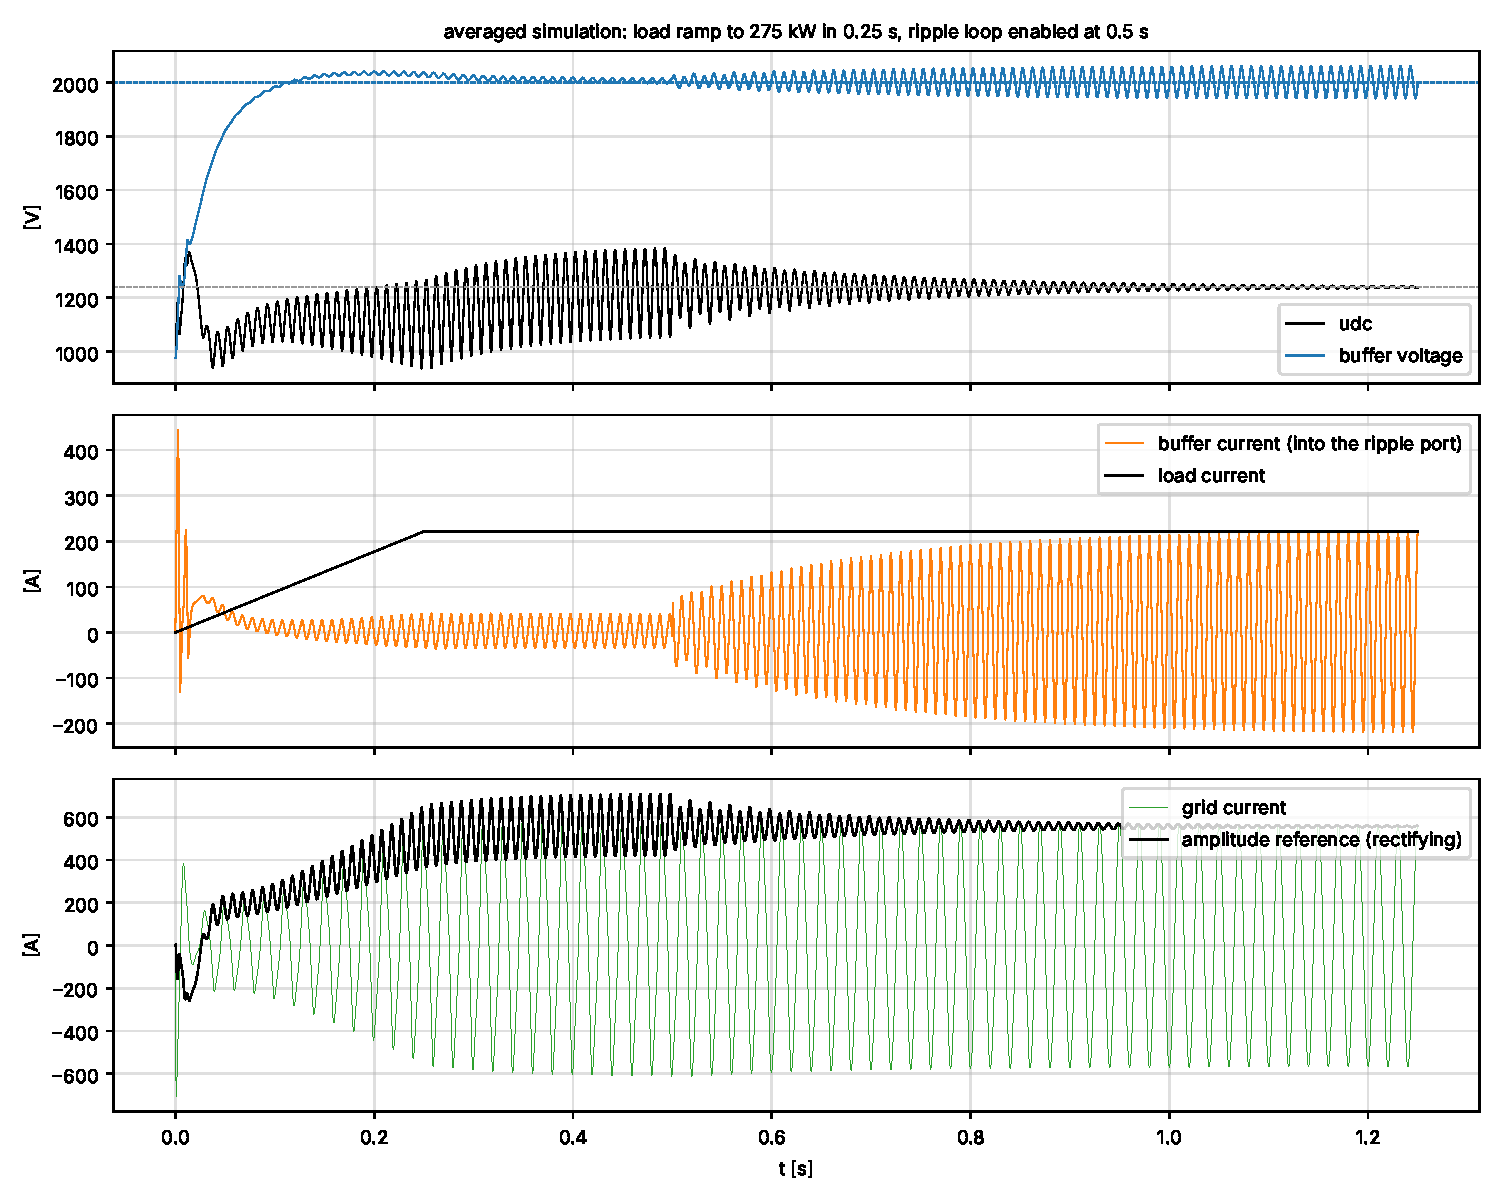
\includegraphics[width=0.95\linewidth]{figures/single_phase_afe_sim_overview.pdf}
	\captionsetup{width=0.92\textwidth, font=small}
	\caption[Averaged simulation, overview.]{Averaged simulation: DC-link and buffer voltages (top), buffer and load currents (middle), grid current and the amplitude reference of the DC-link PI (bottom). The ripple loop is enabled at \SI{0.5}{\second}.}
	\label{fig:overview}
\end{figure}

\begin{figure}[H]
	\centering
	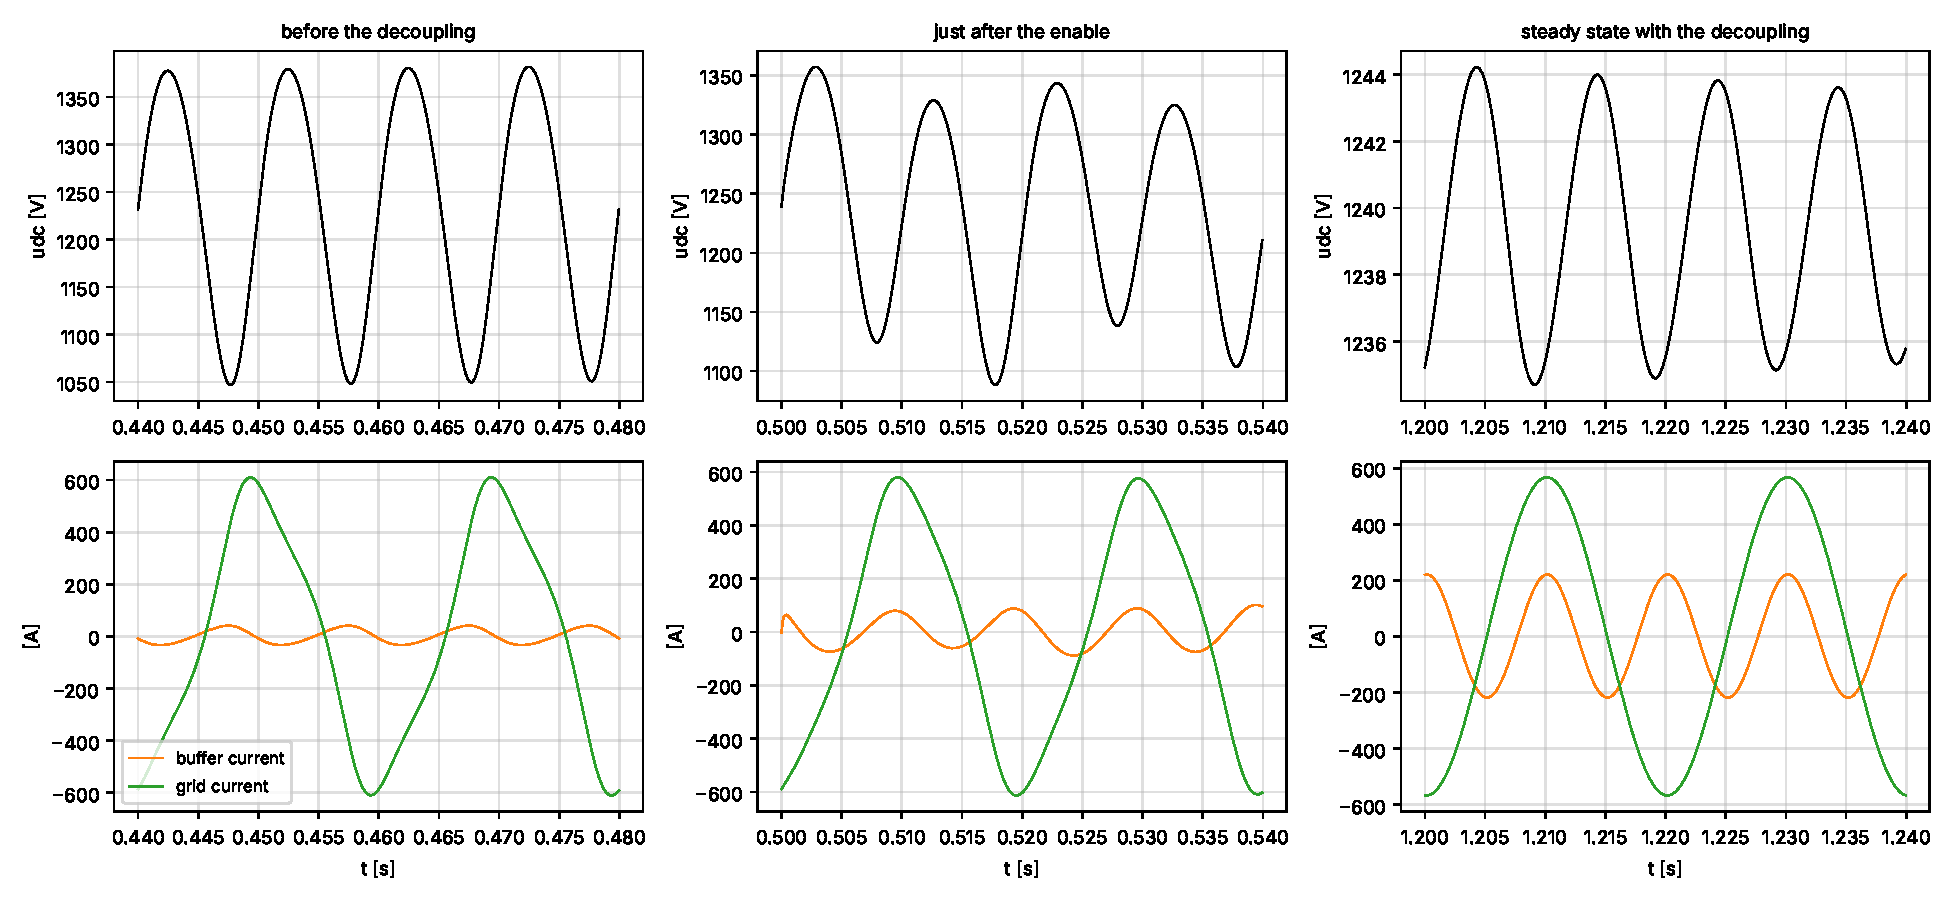
\includegraphics[width=0.98\linewidth]{figures/single_phase_afe_sim_zoom.pdf}
	\captionsetup{width=0.92\textwidth, font=small}
	\caption[Averaged simulation, details.]{Four grid periods before the enable, just after it and in steady state: $u\ped{dc}$ (top), buffer and grid currents (bottom).}
	\label{fig:zoom}
\end{figure}

Before the enable, the DC link ripples by \SI{196}{\volt} (\SI{16}{\percent}, more than the \SI{147}{\volt} of the capacitor alone) and the grid current is visibly distorted: the DC-link PI passes the ripple into the current amplitude reference, which oscillates between \SI{400}{\ampere} and \SI{700}{\ampere} at \SI{100}{\hertz} (Figure~\ref{fig:overview}, bottom). A sinusoid at $\omega$ whose amplitude is modulated at $2\omega$ contains a component at $3\omega$ and one at $\omega$ with another phase: the third harmonic is \SI{13.4}{\percent} of the fundamental and the THD \SI{13.5}{\percent} (Figure~\ref{fig:thd}, left). The extra \SI{50}{\hertz} component also makes the power pulsate more, which is why the ripple is larger than \eqref{eq:ripple}.

After the enable the port current grows to \SI{221}{\ampere} peak at \SI{100}{\hertz}, as \eqref{eq:ib_ref} says for \SI{275}{\kilo\watt}, in about half a second (Figure~\ref{fig:ripple_loop_sim}: the integrators of the vector PI ramp up with the time constant of \eqref{eq:envelope}; \SI{90}{\percent} of the ripple is gone \SI{390}{\milli\second} after the enable). In steady state the DC-link ripple is \SI{9.5}{\volt} (\SI{0.8}{\percent}), the buffer swings by \SI{121}{\volt} peak-to-peak around \SI{2000}{\volt}, the duty of the port moves between 0.60 and 0.64, and the grid current is a clean sinusoid: THD \SI{0.5}{\percent}. The DC-link voltage itself settles at its reference once the ripple no longer disturbs the voltage PI.

\begin{figure}[H]
	\centering
	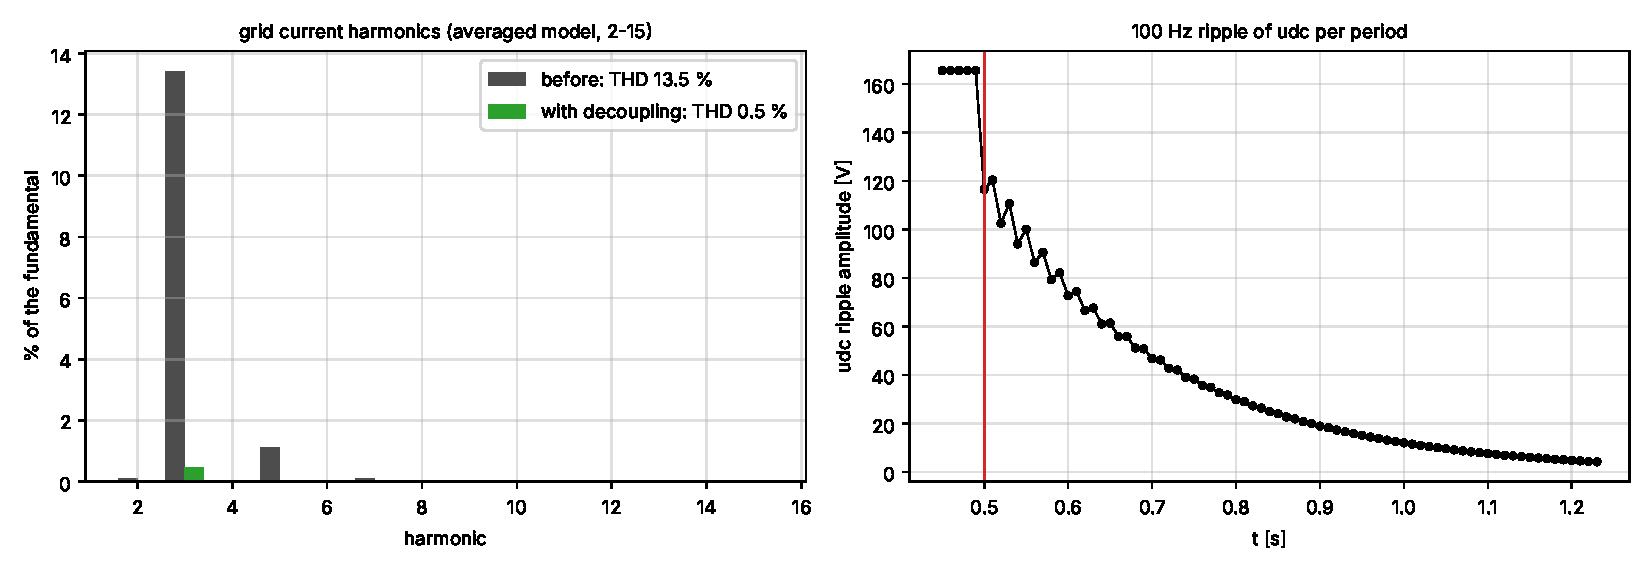
\includegraphics[width=0.98\linewidth]{figures/single_phase_afe_sim_thd_ripple.pdf}
	\captionsetup{width=0.92\textwidth, font=small}
	\caption[Harmonics of the grid current and decay of the ripple.]{Left: harmonics of the grid current before and with the decoupling (averaged model). Right: amplitude of the \SI{100}{\hertz} ripple of $u\ped{dc}$, period by period, around the enable at \SI{0.5}{\second}.}
	\label{fig:thd}
\end{figure}

\begin{figure}[H]
	\centering
	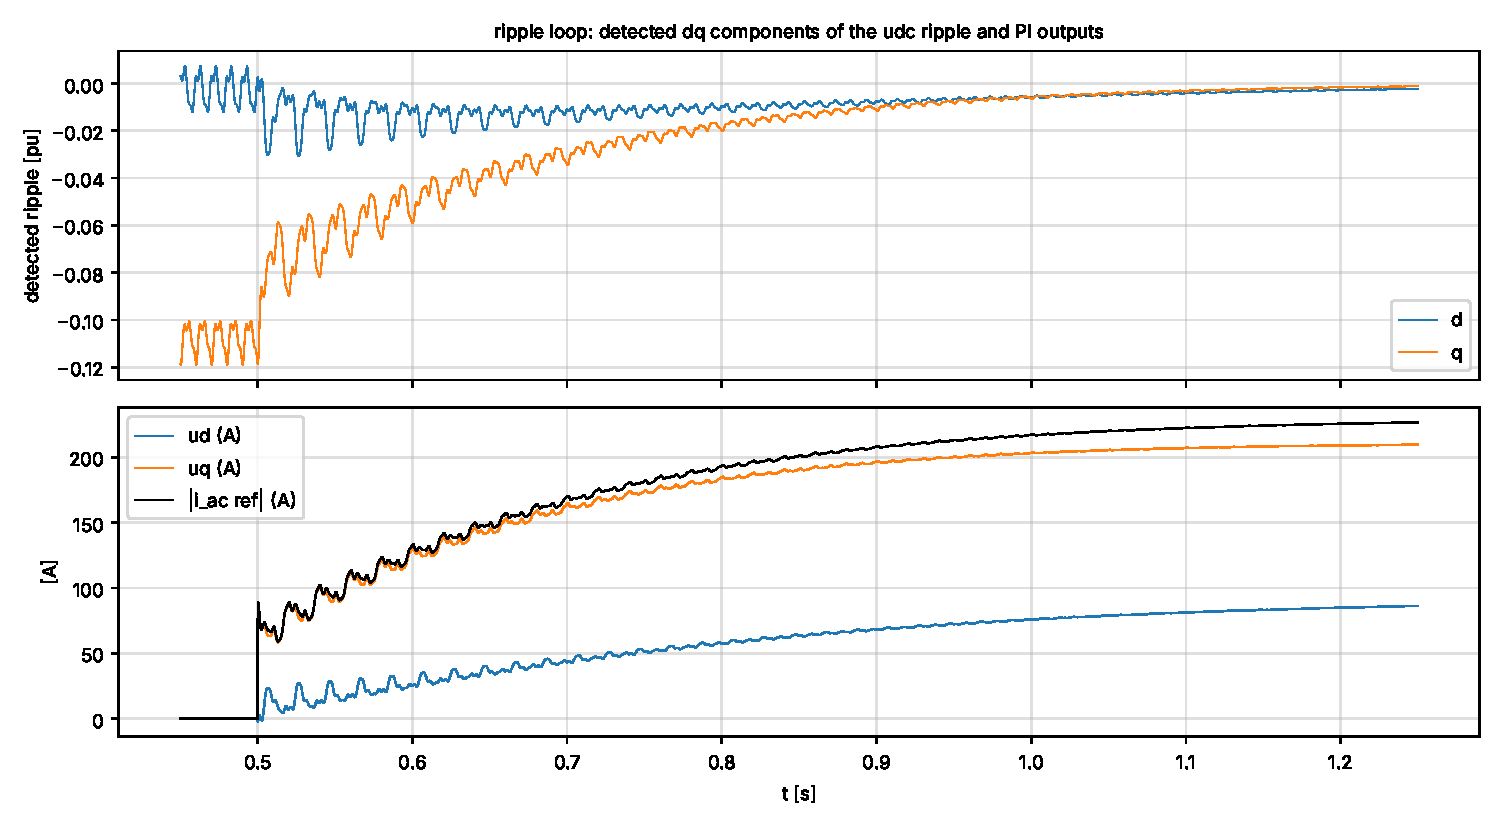
\includegraphics[width=0.95\linewidth]{figures/single_phase_afe_sim_ripple_loop.pdf}
	\captionsetup{width=0.92\textwidth, font=small}
	\caption[Signals of the ripple loop.]{Signals of the ripple loop: the detected $d$ and $q$ components of the ripple (top) and the outputs of the vector PI, in amperes (bottom). The small oscillation on $d$ and $q$ is the residual of other frequencies after the rotation; the integrators average it out.}
	\label{fig:ripple_loop_sim}
\end{figure}

% =============================================================
\section{Check of the numbers of the model}
\label{sec:check}

The script also computes the frequency responses of the four loops with the values of \code{init\_model.m} (Figure~\ref{fig:bode}, Table~\ref{tab:loops}). The delays of the digital control (one control period of computation plus half a period of PWM) are included.

\begin{figure}[H]
	\centering
	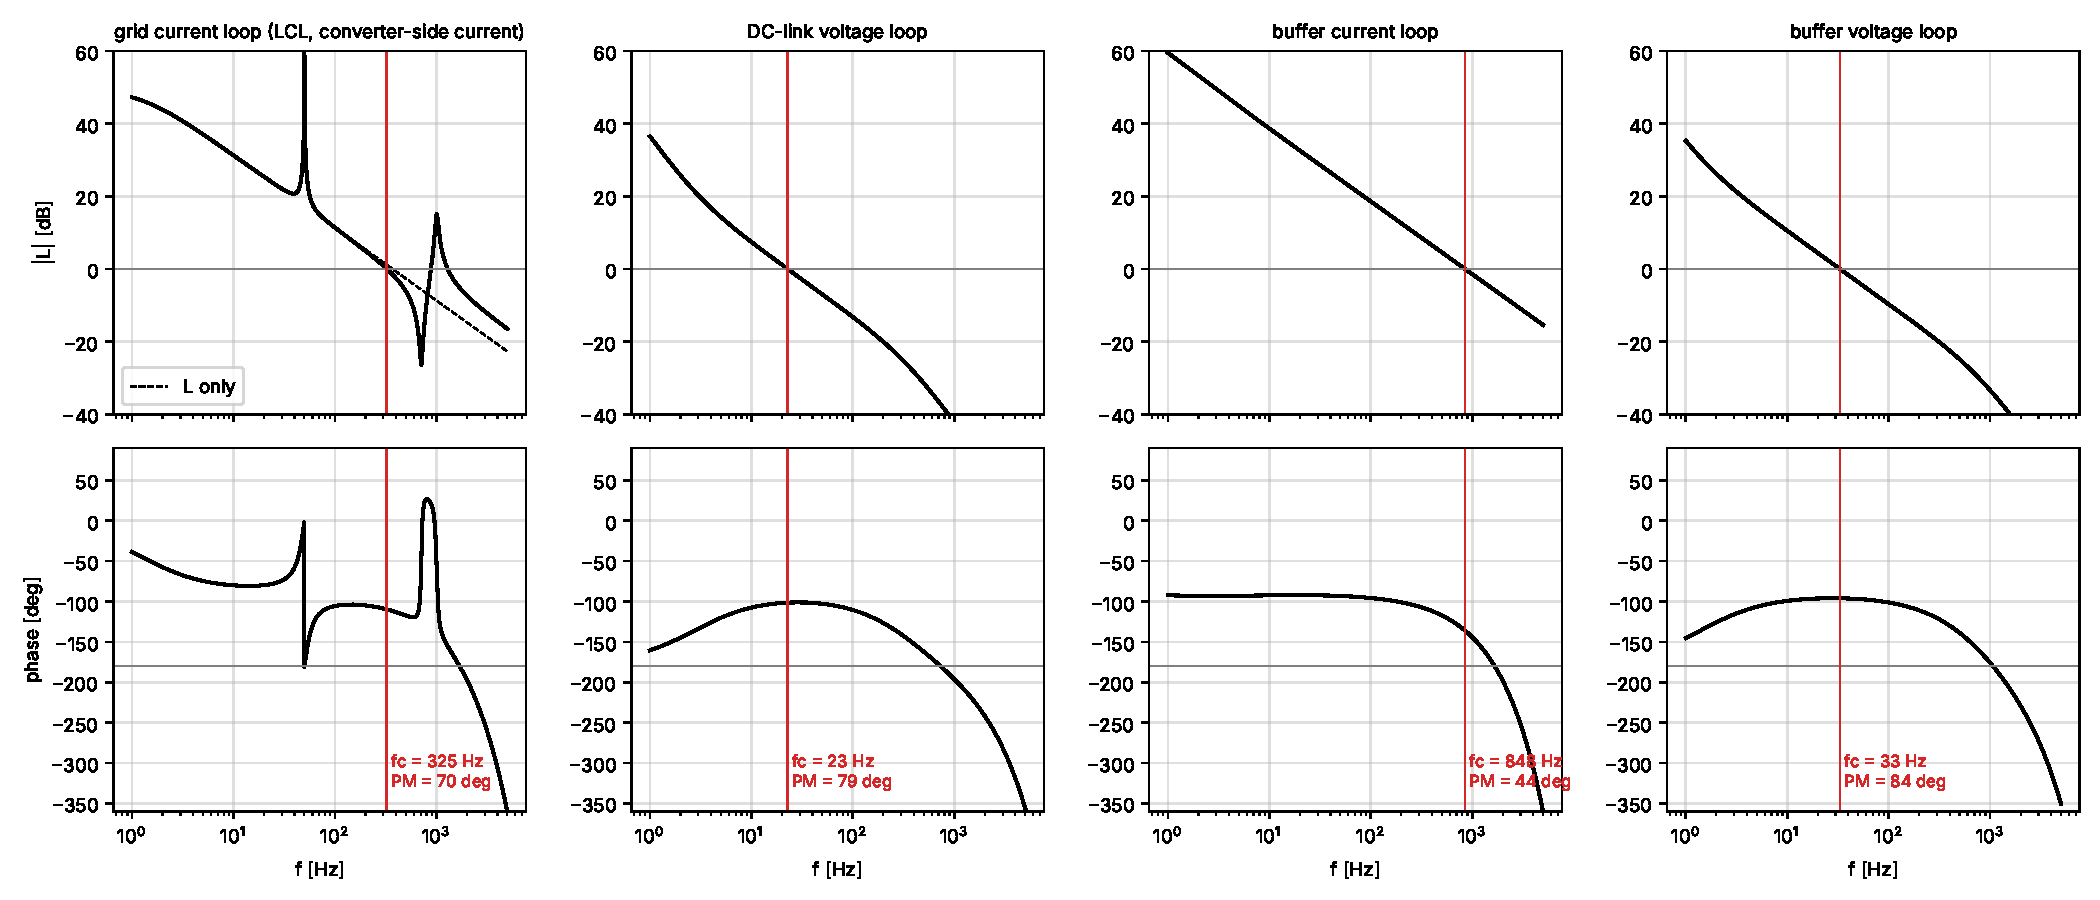
\includegraphics[width=\linewidth]{figures/single_phase_afe_loops_bode.pdf}
	\captionsetup{width=0.92\textwidth, font=small}
	\caption[Open loops of the model.]{Open-loop frequency responses with the gains of the model: grid current loop with the LCL (and with the inductance alone, dashed), DC-link voltage loop, buffer current loop, buffer voltage loop. Red: crossover and phase margin.}
	\label{fig:bode}
\end{figure}

\begin{table}[H]
	\centering
	\captionsetup{width=0.9\textwidth, font=small}
	\caption[Loops of the model.]{Loops of the model: gains and margins.}
	\label{tab:loops}
	\rowcolors{2}{tableShade}{white}
	\begin{tabularx}{0.97\textwidth}{@{} l l l X @{}}
		\toprule
		\textbf{Loop} & \textbf{Gains} & \textbf{Crossover / margin} & \textbf{Note} \\
		\midrule
		grid current & $0.5 / 45$, limit 1 & \SI{325}{\hertz} / \SI{70}{\degree} & LCL resonance at \SI{1007}{\hertz} with \SI{15}{\decibel} of loop gain, gain margin \SI{5.2}{\decibel}; PI zero at \SI{14}{\hertz} \\
		DC-link voltage & $2 / 35$, limit 1.65 & \SI{23}{\hertz} / \SI{79}{\degree} & reference filter \SI{20}{\milli\second}; $|\mathrm{PI}| = 2$ at \SI{100}{\hertz} \\
		buffer current & $1 / 18$, limit 1 & \SI{848}{\hertz} / \SI{44}{\degree} & gain margin \SI{5.9}{\decibel}; at \SI{100}{\hertz}: 1.005, \SI{-6.8}{\degree} \\
		buffer voltage & $2 / 18$, limit 1 & \SI{33}{\hertz} / \SI{84}{\degree} & sees the \SI{100}{\hertz} swing of $u\ped{b}$ \\
		ripple loop & $1 / 18$, limit 1 & pole $-4.3$ \si{\radian\per\second} & chain gain 0.31, phase \SI{-9}{\degree}; \SI{90}{\percent} in \SI{0.4}{\second} \\
		FHT, PLL & $\delta\,0.05$; $1 / 80$ & poles $-\omega$, $-4\omega$ & observer gains $l_1\,0.147$, $l_2\,24.3$ (FHT); $k\ped{x}\,1490$, $k\ped{v}\,\num{3.65e5}$ (ripple observer) \\
		\bottomrule
	\end{tabularx}
	\rowcolors{1}{white}{white}
\end{table}

Three things stand out. The decoupling works and the loops are stable with comfortable margins, except the buffer current loop (\SI{44}{\degree}) and the LCL resonance of the grid current loop, both acceptable. The ripple loop is slow: a time constant of \SI{233}{\milli\second} is fine for a steady load but a load step makes the ripple reappear for about a second; a larger $k\ped{i}$ of the ripple vector PI (the chain is almost a pure gain, so $k\ped{i}$ sets the pole directly: $k\ped{i} = 100$ would give \SI{-24}{\radian\per\second}) or a feed-forward of the pulsating power computed from the measured grid voltage and current would make it fast. And the DC-link voltage loop has no defence against the \SI{100}{\hertz} ripple: when the ripple loop is off, the grid current carries \SI{13}{\percent} of third harmonic.

% =============================================================
\section{Open points}
\label{sec:open}

These are the points found during the check of the model. They are listed here so that they can be decided, not changed silently.

\begin{enumerate}[nosep]
	\item \textbf{Voltage class of the ripple-port bridge.} The buffer is at \SI{2000}{\volt} with a \SI{1700}{\volt} module (\SI{118}{\percent} of its blocking voltage). Options: a lower buffer voltage with a larger swing (\SI{1.79}{\milli\farad} give $\pm\SI{5}{\percent}$ at \SI{2000}{\volt}; at \SI{1500}{\volt}, \SI{3.18}{\milli\farad}), a higher voltage class, or a buck-type port with the buffer below $u\ped{dc}$.
	\item \textbf{Start-up.} The buffer starts at \SI{0}{\volt}: the first milliseconds are a resonant precharge of $C\ped{b}$ through the inductors from a DC link already at the rectified grid peak. Both voltage references (DC link and buffer) ramp from zero while the DC link is already at \SI{976}{\volt}: the DC-link PI asks for an inverting current until the reference passes the measured voltage. A precharge and references that start from the measured values would fix it.
	\item \textbf{Feed-forward of the buffer current loop.} $u\ped{dc,pu}$ instead of $u\ped{dc}/u\ped{b}$ (Section~\ref{sec:control}).
	\item \textbf{Buffer voltage loop at \SI{100}{\hertz}.} It adds a \SI{100}{\hertz} term to the current reference that the ripple loop has to absorb; a notch or a moving average on $u\ped{b}$ would separate the two loops.
	\item \textbf{Speed of the ripple loop.} Time constant \SI{233}{\milli\second}; a larger $k\ped{i}$ or a power feed-forward (Section~\ref{sec:check}).
	\item \textbf{DC-link voltage loop at \SI{100}{\hertz}.} With the ripple loop off the ripple goes into the grid current (\SI{13}{\percent} of third harmonic); a notch at \SI{100}{\hertz} or a moving average over \SI{10}{\milli\second} on $u\ped{dc,pu}$ is the usual cure, at the cost of some phase margin.
	\item \textbf{Dead time.} \SI{1}{\micro\second} against $t\ped{d,off} + t\ped{f} = \SI{1.74}{\micro\second}$ of the module at \SI{125}{\celsius}.
	\item \textbf{Ratings and bases.} The load is \SI{275}{\kilo\watt} on a \SI{225}{\kilo\watt} converter; the per-unit bases are those of the legacy single-phase data set (\SI{838}{\volt}) while the grid peak is \SI{976}{\volt} (\SI{1.164}{pu}); the DC-link voltage scaling of the measurement block was \SI{1070}{\volt} against $u\ped{dc,nom} = \SI{1239.4}{\volt}$ (now both read \code{param.afe.hw.udc\_nom}).
	\item \textbf{PLL and grid.} The PLL reads the three phase voltages of the emulator while the converter is single-phase; a single-phase PLL (SOGI or FHT on $u\ped{ab}$) would match the hardware. The grid has no impedance (no line inductance, no transformer): the LCL resonance and the PLL are not tested against a weak grid.
\end{enumerate}

% =============================================================
\section{How to run}
\label{sec:run}

\begin{enumerate}[nosep]
	\item Put the \code{library} repository on the MATLAB path with subfolders.
	\item From the model folder run \code{init\_model.m}: it fills the struct \code{param} (one group per subsystem, listed in the \code{README.md} of the folder), opens \code{single\_phase\_afe.slx} and checks that every \code{param.*} name read by the model exists. The parameter functions are in \code{private/} and are visible only from the model folder.
	\item Simulate (\SI{1.25}{\second}) and run \code{plotting\_results\_sim\_results.m}.
	\item The numbers and the figures of this note come from the script \path{single_phase_afe_design_check.py}, run with Python~3 (numpy, scipy, matplotlib) from its folder; the option \code{--no-sim} skips the averaged simulation.
\end{enumerate}

% =============================================================
\section{Conclusions}
\label{sec:conclusions}

The model \code{single\_phase\_afe} implements active power decoupling with a ripple port: a second full bridge, two inductors and a buffer capacitor that swings around \SI{2000}{\volt}. The method is a closed loop on the ripple itself: an observer isolates the \SI{100}{\hertz} ripple of the DC-link voltage, a phase-shift filter builds its quadrature, a rotation at twice the grid angle turns it into two constants, a vector PI drives them to zero, and the output is applied through the $\beta$ axis so that the \SI{90}{\degree} of the DC-link capacitor are compensated. In the averaged simulation the ripple falls from \SI{16}{\percent} to below \SI{1}{\percent} and the third harmonic of the grid current from \SI{13}{\percent} to \SI{0.5}{\percent}, in about half a second. The open points of Section~\ref{sec:open} are for the next revision of the model.

% =============================================================
\section{Files}
\label{sec:files}

\begin{table}[H]
	\centering
	\captionsetup{width=0.9\textwidth, font=small}
	\caption[Files.]{Files of the model and of this note.}
	\label{tab:files}
	\rowcolors{2}{tableShade}{white}
	\begin{tabularx}{0.97\textwidth}{@{} l X @{}}
		\toprule
		\textbf{File} & \textbf{Content} \\
		\midrule
		\multicolumn{2}{@{}p{\dimexpr0.97\textwidth-2\tabcolsep\relax}@{}}{\textbf{folder \path{foundations_of_power_electronics/single_phase_afe/} of \code{modelization-and-control}}} \\
		\code{single\_phase\_afe.slx} & the model: grid emulator, LCL, the two bridges with the IGBT loss and thermal models, DC link, load, control \\
		\code{init\_model.m}, \code{private/} & initialization (struct \code{param}) and its parameter functions; \code{README.md} describes the folder, the parameter groups and the open points \\
		\code{claude\_analysis/} & \path{single_phase_afe_design_check.py}, its printed output and the figures of this note \\
		\midrule
		\multicolumn{2}{@{}p{\dimexpr0.97\textwidth-2\tabcolsep\relax}@{}}{\textbf{C sources of the library}, folder \path{library/user_defined_functions/ccaller/src/}} \\
		\path{linear_double_integrator_observer.c}, \path{phase_shift_flt.c} & the observer of Step~1 and the phase-shift filter of Step~2 (FHT and vector PI: \path{first_harmonic_tracker.c}, \path{dqvector_pi.c}; the model uses their Simulink versions) \\
		\midrule
		\multicolumn{2}{@{}p{\dimexpr0.97\textwidth-2\tabcolsep\relax}@{}}{\textbf{this note}: \path{repos_doc/single_phase_afe_power_decoupling/} of \code{repositories-documentation}, copy in \path{library/documentation/single_phase_afe_power_decoupling/} of \code{library}} \\
		\path{single_phase_afe_power_decoupling.tex}, \code{.pdf} & source and PDF \\
		\path{single_phase_afe_design_check.py}, \code{figures/} & the script and the PDF figures it produces \\
		\bottomrule
	\end{tabularx}
	\rowcolors{1}{white}{white}
\end{table}

% =============================================================
\begin{thebibliography}{99}
	\bibitem{model_repo} pwr-control, \textit{modelization-and-control} repository, \url{https://github.com/pwr-control/modelization-and-control}, folder \path{foundations_of_power_electronics/single_phase_afe}.
	\bibitem{library_repo} pwr-control, \textit{library} repository (Simscape components, C-Caller sources and documentation), \url{https://github.com/pwr-control/library}.
	\bibitem{krein2012} P.~T. Krein, R.~S. Balog, and M.~Mirjafari, ``Minimum energy and capacitance requirements for single-phase inverters and rectifiers using a ripple port,'' \emph{IEEE Trans. Power Electron.}, vol.~27, no.~11, pp.~4690--4698, Nov. 2012.
	\bibitem{sun2016} Y.~Sun, Y.~Liu, M.~Su, W.~Xiong, and J.~Yang, ``Review of active power decoupling topologies in single-phase systems,'' \emph{IEEE Trans. Power Electron.}, vol.~31, no.~7, pp.~4778--4794, July 2016.
	\bibitem{hu2013} H.~Hu, S.~Harb, N.~Kutkut, I.~Batarseh, and Z.~J. Shen, ``A review of power decoupling techniques for microinverters with three different decoupling capacitor locations in PV systems,'' \emph{IEEE Trans. Power Electron.}, vol.~28, no.~6, pp.~2711--2726, June 2013.
	\bibitem{wang2011} R.~Wang, F.~Wang, D.~Boroyevich, R.~Burgos, R.~Lai, P.~Ning, and K.~Rajashekara, ``A high power density single-phase PWM rectifier with active ripple energy storage,'' \emph{IEEE Trans. Power Electron.}, vol.~26, no.~5, pp.~1430--1443, May 2011.
	\bibitem{teodorescu2011} R.~Teodorescu, M.~Liserre, and P.~Rodr\'iguez, \emph{Grid Converters for Photovoltaic and Wind Power Systems}. Wiley-IEEE Press, 2011.
	\bibitem{sp_note} D.~Bagnara, \textit{Single-Phase Grid-Tied T-Type Inverter: model, control design and discrete implementation}, pwr-control technical note, Rev.~01, October 2026, \path{repos_doc/single_phase_grid_tied_inverter_analysis} of \url{https://github.com/pwr-control/repositories-documentation} (first harmonic tracker and vector PI on a single-phase current).
\end{thebibliography}

\end{onehalfspace}
\end{document}
